\chapter{Detecting memory access behavior in STM applications}\label{chap:mechanism}

In this chapter, a mechanism to detect the sharing behavior of STM applications is proposed. It is the base mechanism used in all thesis contributions.

\section{Overview}

Detecting the memory access behavior is the first step to perform a sharing-aware thread mapping. It is necessary to know which memory address is being accessed and which thread is accessing it. In shared memory programming models, communication is implicit, i.e., it is performed through access to shared memory areas. This characteristic adds more challenge to detect the memory access behavior in shared memory architectures.

Detecting the communication behavior accurately with tools such as \texttt{numalize}~\cite{Diener2015} cause high overheads. Hence, it necessary to use a heuristic to detect communication events accurately and with low overhead. A \emph{communication event} happens when at least 2 threads access the same shared variable. Although writes to memory are more expensive, i.e., they imply in cache invalidation and interconnection traffic between remote notes, we will not differentiate reads from writes in the proposed mechanism. Besides, we will take into consideration the operations performed by all transactions, including aborted. If one transaction aborts, it is accessing shared variables with other transactions. If we take into consideration only committed transactions, this relationship would not be registered, making the mechanism less precise. Also, it is important to have a heuristic to avoid false temporal communication, i.e., two threads access the same shared variable but in long difference execution intervals. In that case, during the second access, the first one already has been evicted from the cache lines.

To store the amount of communication between pairs of threads, we use a communication matrix (Section~\ref{sect:commMatrix}), where each matrix position represents the amount of communication between pairs of threads. Since access to a shared variable from the same thread does not represent a communication event, matrix diagonals are zero.

\section{Mechanism}

The main idea of this mechanism is to work inside the STM library, by only keeping track of STM accesses. To detect the memory access behavior of an application, it is necessary to know which addresses the application is accessing. In STM runtimes, each transactional data access operation explicitly includes the addresses used in the operation. For instance~\cite{Harris:2010}:

 \begin{center}
 	\lstinputlisting[language=STM, framerule=0pt, xleftmargin=6em, numbers=none]{code/dataAccess.c}
 \end{center}

As this is already available to the STM runtime, it is not necessary to rely on external tools or add instrumentation overhead to get this information.  Besides, the STM runtime knows which thread is performing the access. Since STM runtimes have precise information about shared variables, it is possible to determine the communication behavior by tracking transactional reads and writes instead of tracking all memory accesses. Our detection mechanism works as follows. When at least 2 distinct threads access the same address, a communication event between them is updated in a communication matrix. %The amount of communication between threads is stored in a communication matrix. %, where each matrix position represents the amount of communication between pairs of threads. 

\begin{figure}[!ht]
%https://docs.google.com/presentation/d/1vP4mTZYlR-y3ibKTqbjXApHYswgchvwL0obU7SrQkMI/edit?usp=sharing
	\centering
	\fbox{
		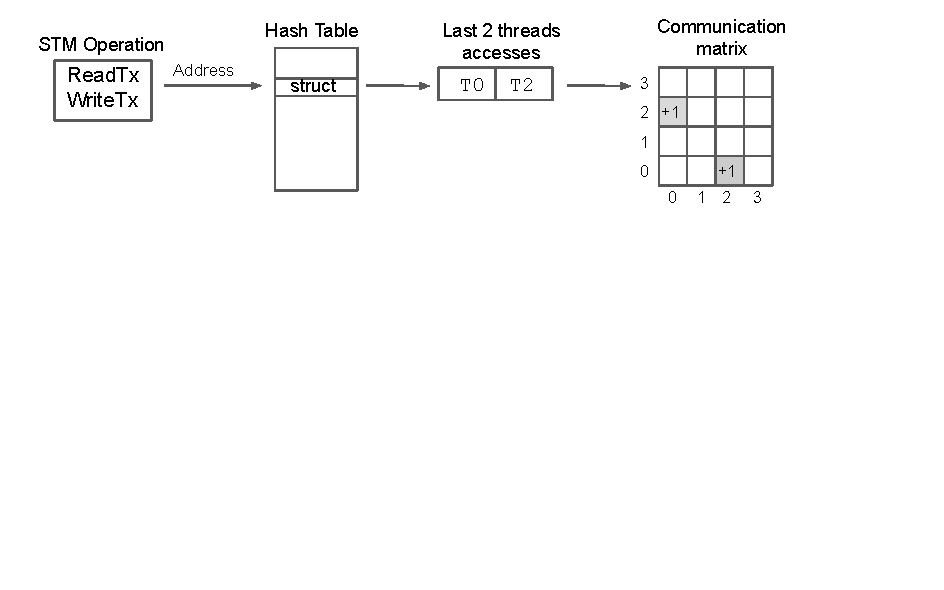
\includegraphics[width=\fullImageWidth\textwidth,trim=10 170 60 0,clip]{figures/mechanism/mechanism.pdf}
	}
	\caption{Mechanism for detecting communication patterns. Data structures are shown for an application consisting of 4 threads (0-3.)}
	\label{fig:mechanism}
\end{figure}


\begin{figure}[!ht]
	%https://docs.google.com/presentation/d/1PTBP2GqremN_1nalfXQhCORR1nwgsHspnoNh1o6fKCI/edit#slide=id.g961e369ddb_3_0
	\centering
	\fbox{
		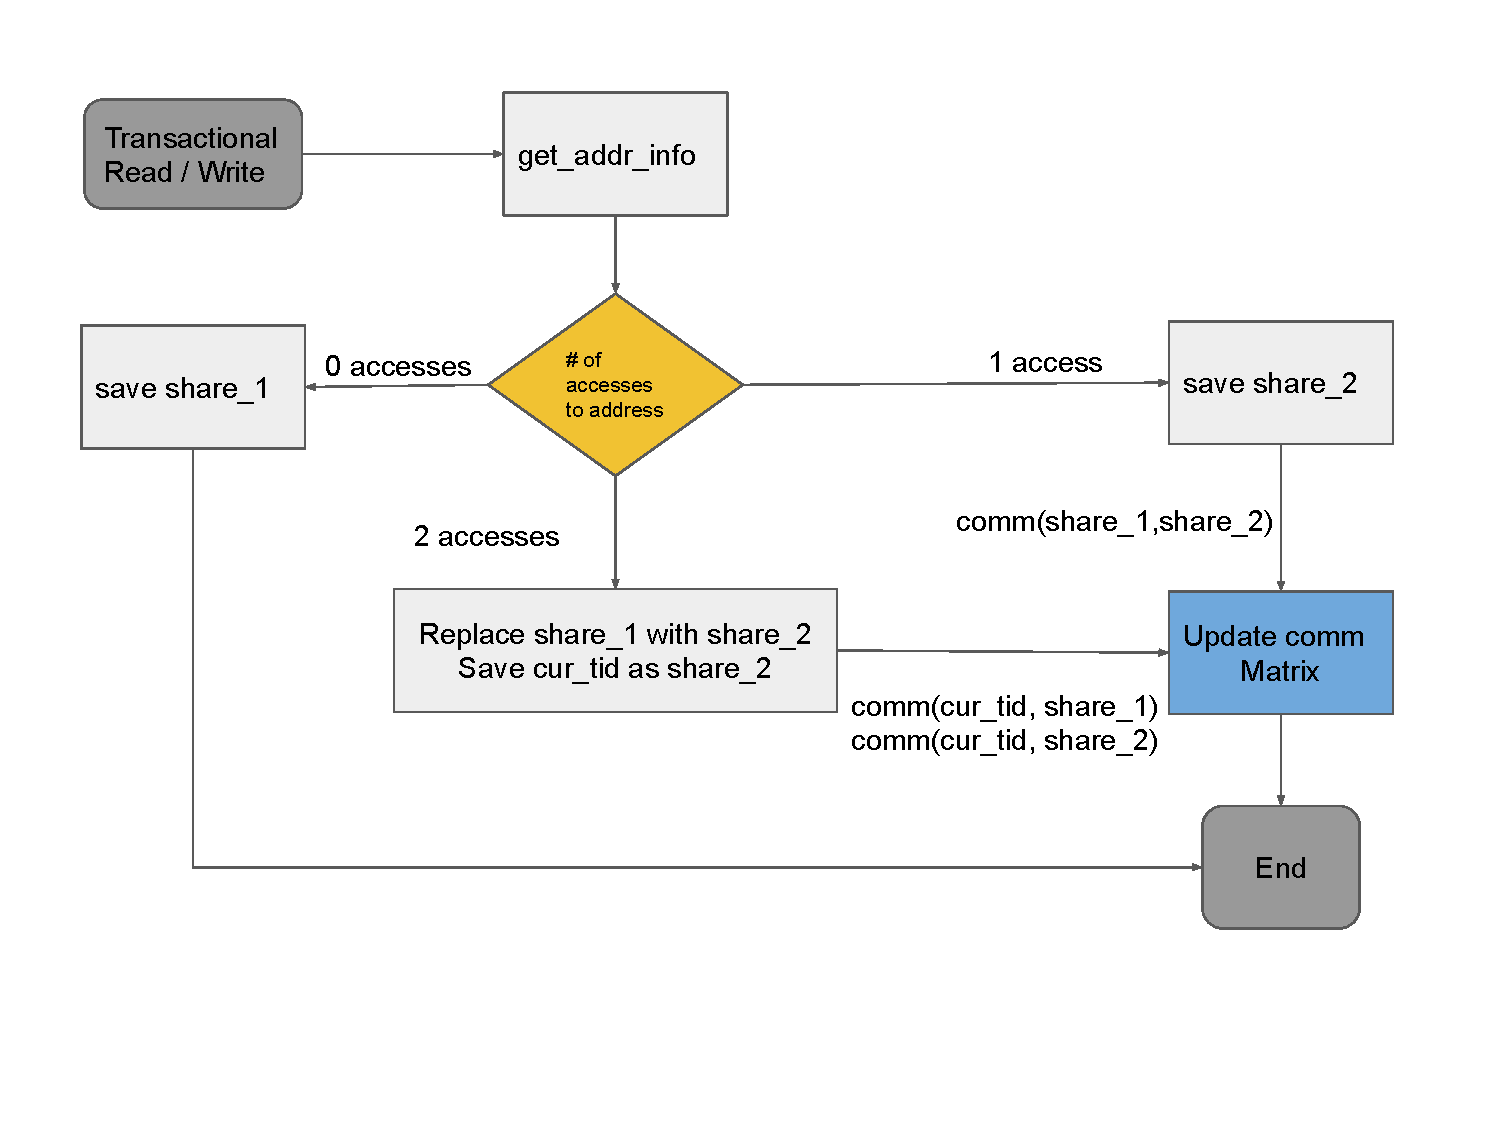
\includegraphics[width=\fullImageWidth\textwidth,trim=20 80 30 30,clip]{figures/mechanism/mechanism-fluxogram.pdf}
		%		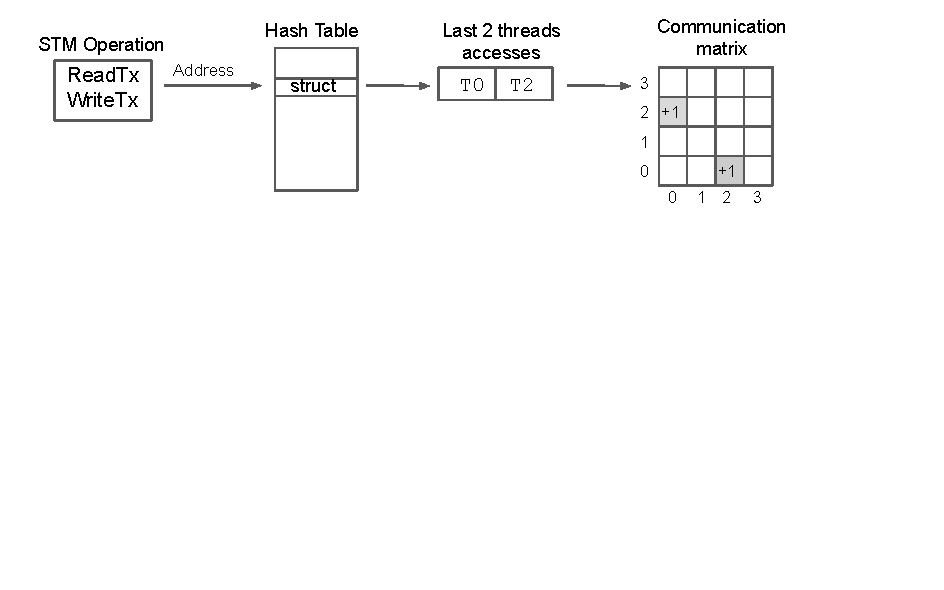
\includegraphics[width=\fullImageWidth\textwidth]{figures/mechanism/mechanism.png}
	}
	\caption{Flowchart of the proposed mechanism.}
	\label{fig:mechanism-fluxogram}
\end{figure}

\begin{algorithm}[!ht]
	\caption{Detecting communication patterns.}\label{alg:detectcomm}
%	\small
	\begin{algorithmic}[1]
		\Require
		\Statex \textbf{addr}: memory address being accessed
		\Statex \textbf{tid}: thread ID of the thread that is accessing the address
		\Statex
		\LineComment{\texttt{elem} is a struct that stores the memory address and the last 2 threads that have accessed it}
		\State $elem \gets \text{getAddressInfo}(addr)$ \label{alg1:elem}
		\State $accesses \gets \text{getAccesses}(elem)$ \label{alg1:count}
		\If {$(accesses = 0)$} \Comment{First access to the address} \label{alg1:0acc}
		\State $elem.t1 \gets tid$ \label{alg1:0accStore}
		% \EndIf
		\ElsIf {($accesses = 1$)}  \Comment{One previous access} \label{alg1:1acces}
		\If {($elem.t1 \neq tid$)} \label{alg1:1accesDiff}
		\State $\text{update\_comm\_matrix}(tid, \ elem.t1)$ \label{alg1:1accesComm}
		\State $elem.t2 \gets elem.t1$ \label{alg1:1accest2}
		\State $elem.t1 \gets tId$ \label{alg1:1accest1}
		% \EndIf
		\EndIf
		\ElsIf {($accesses = 2$)} \Comment{Two previous accesses} \label{alg1:2acces}
		\If {($elem.t1 \neq tid$)  \textbf{and} ($elem.t2 \neq tid$)} \label{alg1:2acces2diff}
		\State $\text{update\_comm\_matrix}(tid, \ elem.t1)$ \label{alg1:2acces2diffupt1}
		\State $\text{update\_comm\_matrix}(tid, \ elem.t2)$ \label{alg1:2acces2diffupt2}
		\State $elem.t2 \gets elem.t1$ \label{alg1:2acces2diffdel}
		\State $elem.t1 \gets tid$
		\ElsIf {($elem.t1 = tid$)} \label{alg1:2acces1difft2}
		\State $\text{update\_comm\_matrix}(tid, \ elem.t2)$
		\ElsIf {($elem.t2 = tid$)} \label{alg1:2acces1difft1}
		\State $\text{update\_comm\_matrix}(tid, \ elem.t1)$
		\State $elem.t2 \gets elem.t1$ \label{alg1:2acces1difft1del}
		\State $elem.t1 \gets tid$
		% \EndIf
		\EndIf
		\EndIf
	\end{algorithmic}
\end{algorithm}

Our mechanism to detect the communication pattern of an application is shown in Figures~\ref{fig:mechanism}--\ref{fig:mechanism-fluxogram} and detailed in Algorithm~\ref{alg:detectcomm}. This mechanism is executed before each transactional read or write operation. To keep track of accessed addresses, a hash table is used, in which keys are memory addresses. Each position of the hash table contains a structure with the memory address and the last 2 threads that have accessed it. Following the intuition of previous work, we store only the last 2 thread access, to avoid false temporal communication~\cite{Diener:2016:2}. In case of hash conflicts, a linked list with all memory addresses with the same hash is kept. In line~\ref{alg1:elem}, the function \texttt{getAddressInfo} gets from the hash table the structure containing information about the address being accessed. The next step is to get how many accesses this address had before the current one (line \ref{alg1:count}). If it is the first access (line \ref{alg1:0acc}), we only store the thread that is accessing it (line \ref{alg1:0accStore}), i.e., no communication events have happened yet. The next case is if the address had one access before the current (line \ref{alg1:1acces}) and it was made by a different thread (line \ref{alg1:1accesDiff}). If true, we have a communication event. In that case, we call the function \texttt{update\_comm\_matrix} (line \ref{alg1:1accesComm}) to update the communication matrix, increasing the amount of communication between the two threads. The matrix is square and symmetric because the amount of communication, for instance, between threads 0 and 2 is the same from 2 and 0 (\figurename~\ref{fig:mechanism}). Also, the matrix has an order equal to the maximum number of threads. Using the matrix, we update the threads that accessed the address (lines \ref{alg1:1accest2} and \ref{alg1:1accest1}). It is worth noting that write accesses to the communication matrix are not synchronized. This decision was made because the high overhead involved to synchronize the access. Besides, the collateral effects expected due to the parallel updates on the matrix, for instance, incorrect pairs of thread being incorrectly updated in the matrix, are considered eventual and not harmful to the mechanism.

The final case is if the address had 2 previous accesses (line \ref{alg1:2acces}), then there are 3 sub-cases. The first one is if the current thread accessing the address is different from the 2 previous (line \ref{alg1:2acces2diff}). In that case, we have a third distinct thread accessing the address, and we update the communication matrix between the 3 (lines \ref{alg1:2acces2diffupt1} and \ref{alg1:2acces2diffupt2}). After that, the oldest access is removed (line \ref{alg1:2acces2diffdel}). However, if the test of the line \ref{alg1:2acces2diff} was false, it means that the current thread accessing the address is the same from a previous one. In that case, we need to check which thread is accessing again (lines \ref{alg1:2acces1difft2} and \ref{alg1:2acces1difft1}), and update the communication matrix correctly. Also, since we keep only the last 2 accesses to the memory address, when a third thread access the address, it is necessary to replace the oldest one (line \ref{alg1:2acces1difft1del}).

\section{Implementation}\label{sec:implement}

We implemented our proposed mechanism inside the state-of-art STM library \texttt{TinySTM}~\cite{TinySTM2}, version 1.0.5. The majority of the modifications were made in the file \texttt{stm\_internal.h}. The Algorithm~\ref{alg:detectcomm} is called inside the functions \texttt{stm\_write} and \texttt{stm\_load} from \texttt{TinySTM}. 

\section{Evaluation}

This section describes experiments made in order to evaluate the proposed mechanism to detect the sharing behavior of STM applications.

\subsection{Methodology}\label{sec:mechMethodology}

We used the proposed mechanism to collect the communication matrices of STM applications by using the modified version of the \texttt{TinySTM} library (Section~\ref{sec:implement}), with the default options: \emph{lazy} version management, \emph{eager} conflict detection and contention manager \emph{suicide}.

\begin{table}[!tb]
	\small
	\centering
	\caption{Default arguments for the programs used in the experiments.}
	\label{tab:defaultParams}
	\begin{tabularx}{\textwidth}{@{}lXl@{}}
		\toprule
		Application & Arguments                                          \\ \midrule
		bayes                & \texttt{-v32 -r8192 -n10 -p40 -i2 -e8 -s1 -t \thNumber}                \\
		genome               & \texttt{-g49152 -s256 -n33554432 -t \thNumber}                         \\
		intruder             & \texttt{-a10 -l128 -n262144 -s1 -t \thNumber}                          \\
		kmeans               & \texttt{-m40 -n40 -t0.00001 -i random-n65536-d32-c16.txt -p \thNumber}\\
		labyrinth            & \texttt{-i random-x1024-y1024-z9-n1024.txt -t \thNumber}               \\
		ssca2                & \texttt{-s21 -i1.0 -u1.0 -l3 -p3 -t \thNumber}                         \\
		vacation             & \texttt{-n4 -q90 -u100 -r1310720 -t16777216 -c \thNumber}              \\
		yada                 & \texttt{-a15 -i ttimeu1000000.2 -t \thNumber}                          \\
		redblacktree			& \texttt{-u 20 -i 1000000 -d 500000000 -n \thNumber}                          \\
		hashmap			& \texttt{-u 20 -i 1000000 -d 500000000 -n \thNumber}                          \\
		\bottomrule
	\end{tabularx}
\end{table}

The applications used in the experiments were all eight benchmarks from the Stanford Transactional Applications for Multi-Processing (\texttt{STAMP})~\cite{STAMP} version 0.9.10, and two micro-benchmarks (HashMap and Redblacktree) from \citeNamesYearPar{Diegues:2014:2}. The input arguments used to run each application are shown in \tablename~\ref{tab:defaultParams}. Most parameters are larger than the largest ones suggested in the original paper~\cite{STAMP} to achieve more substantial execution times on modern machines. To run the experiments, we used the the following NUMA machine (node distances were gathered with \texttt{numactl}~\cite{libnuma}):

\begin{itemize}
	\item \textbf{Xeon}: 8 Intel Xeon E5-4650 processors and 488 GiB of RAM running Linux kernel 4.19.0-9. Each CPU has 12 2-HT cores, totaling 96 cores. Each CPU corresponds to a NUMA node (for a total of 8 NUMA nodes), and 12$\times$ 32 KB L1d, 12$\times$ 32 KB L1i, 12$\times$ 256 KB L2 and 30 MB L3 cache. Node distances: 50 -- 65. Applications were compiled using gcc 8.3.0.
\end{itemize}

\subsection{Communication matrices}\label{sect:StampMatrices}
Figures~\ref{fig:commMatrOpt16}--\ref{fig:commMatrXeon96} shown the collected communication matrices using the proposed mechanism for 16, 32, 64 and 96 threads. In the figures, axes show threads IDs and darker cells indicate more communication between pairs of threads.
\begin{figure}[ht]
	\centering
	\subfigure[bayes]{
		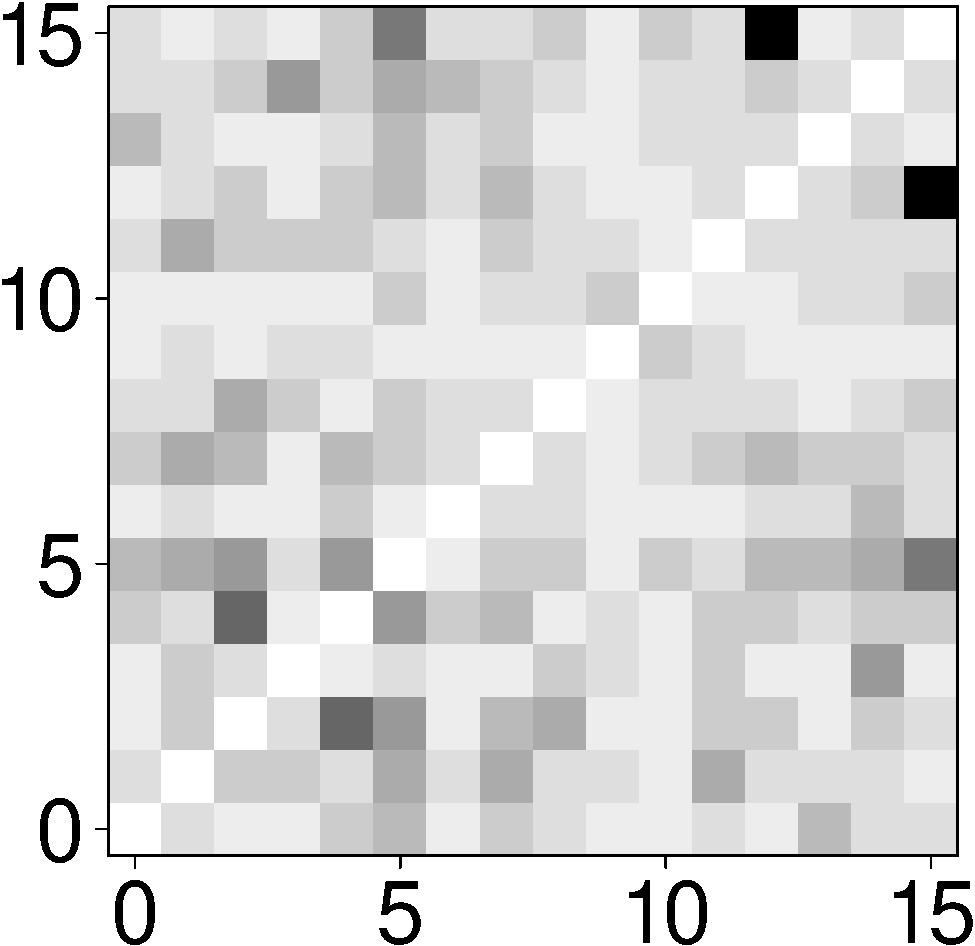
\includegraphics[width=\oneFPage\textwidth]{figures/mechanism/matrices/opteron/bayes_16.pdf}
	}
	\subfigure[genome]{
		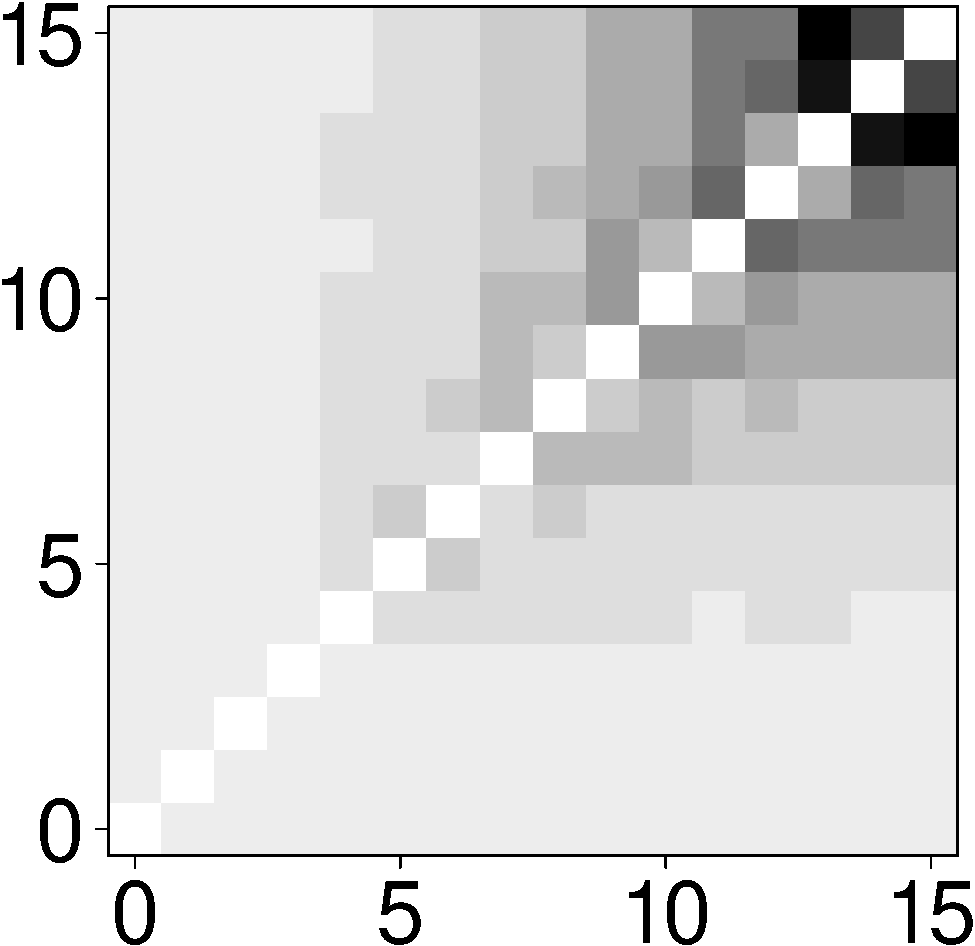
\includegraphics[width=\oneFPage\textwidth]{figures/mechanism/matrices/opteron/genome_16.pdf}
	}
	\subfigure[intruder]{
		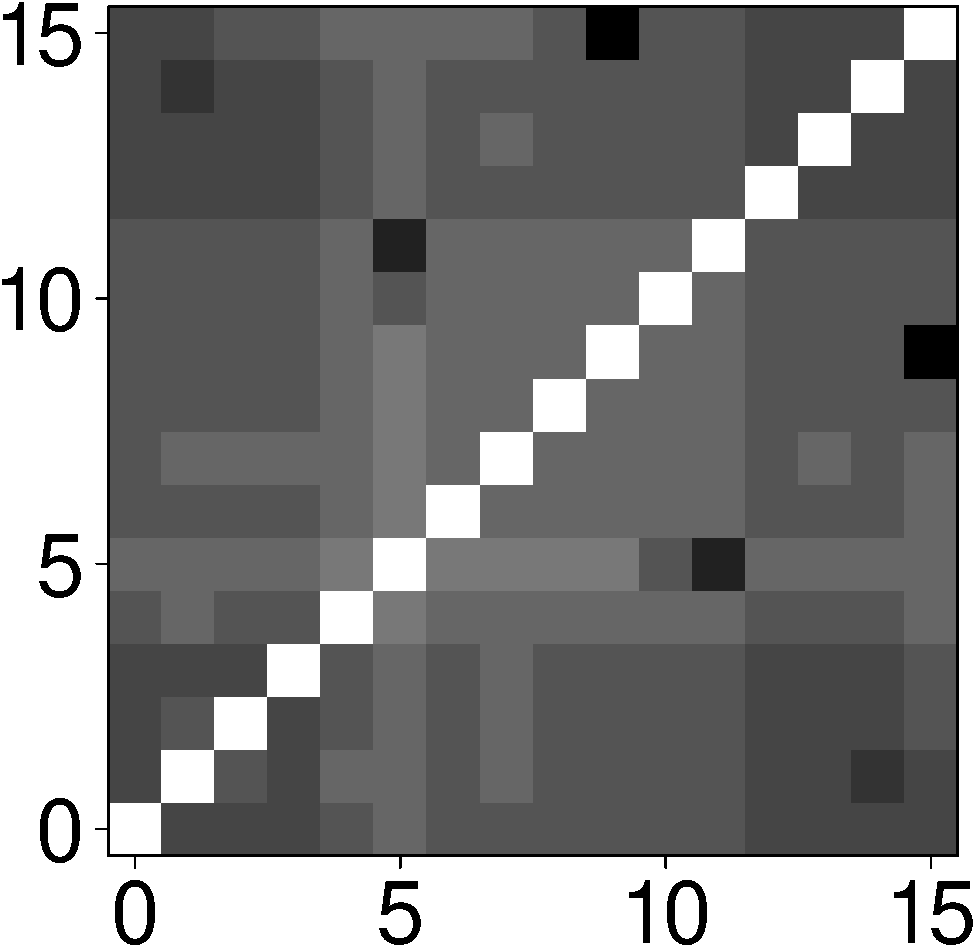
\includegraphics[width=\oneFPage\textwidth]{figures/mechanism/matrices/opteron/intruder_16.pdf}
	}
	\subfigure[kmeans]{
		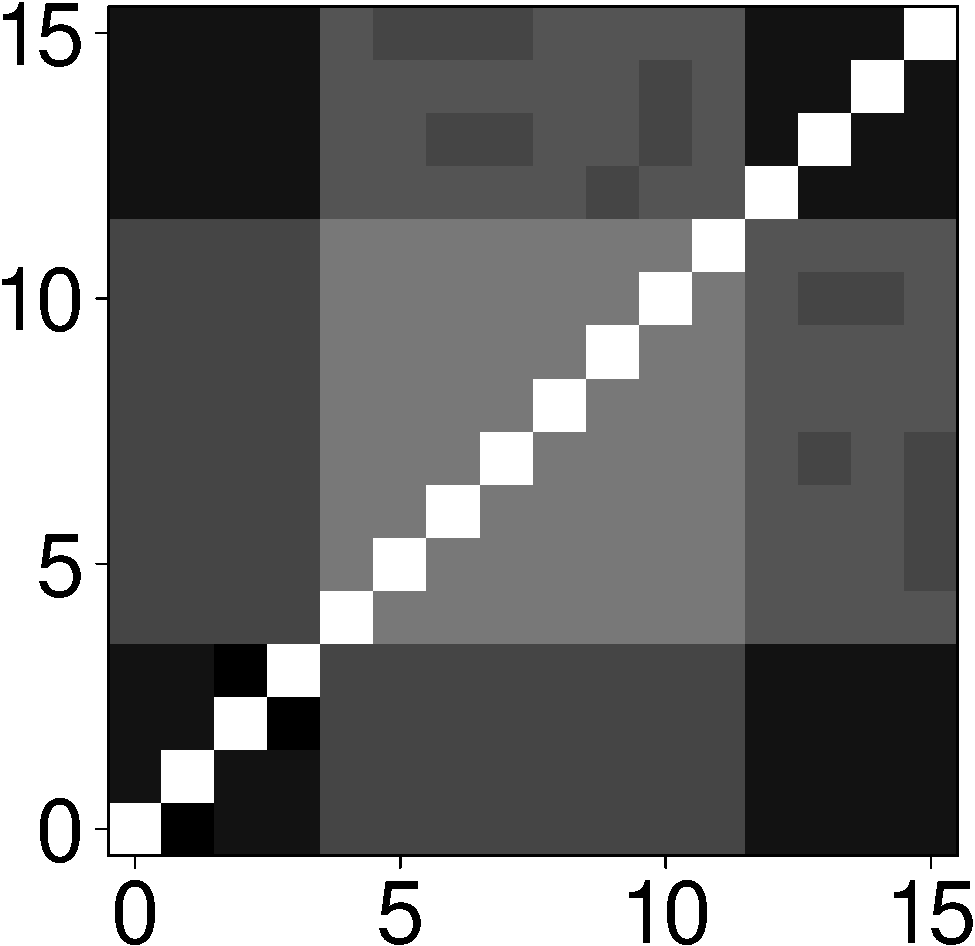
\includegraphics[width=\oneFPage\textwidth]{figures/mechanism/matrices/opteron/kmeans_16.pdf}
	}
	\subfigure[labyrinth]{
		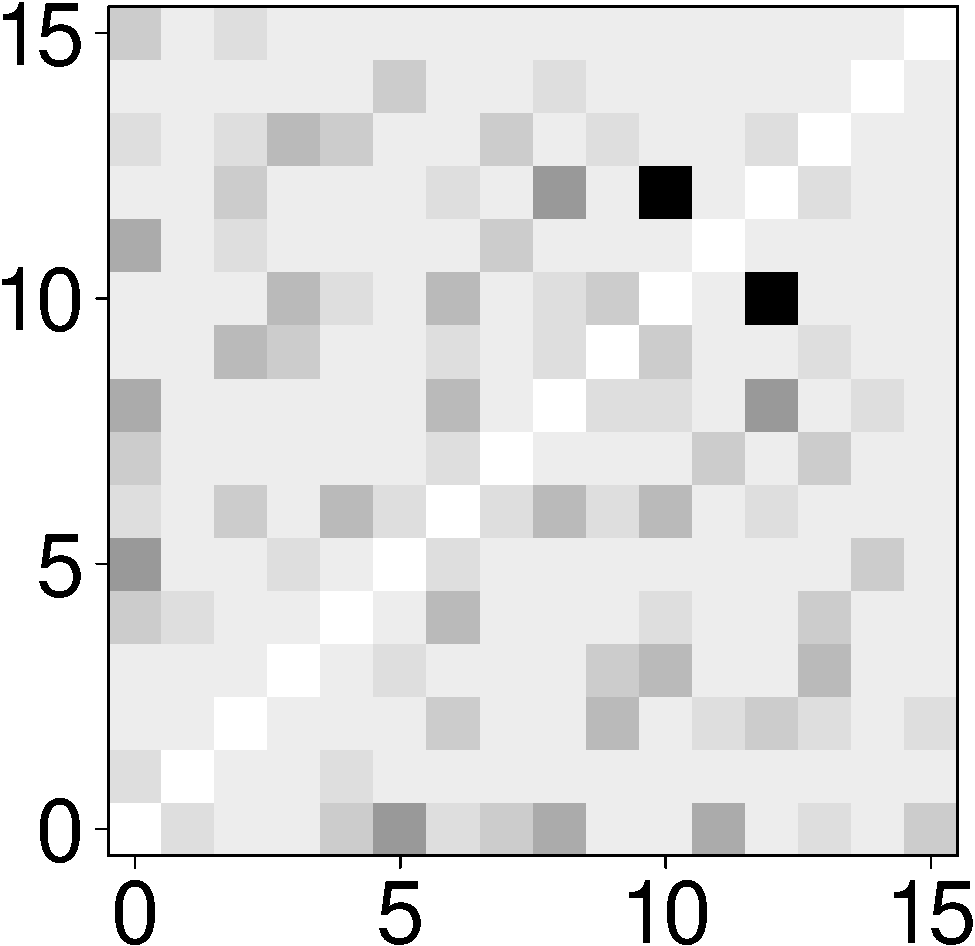
\includegraphics[width=\oneFPage\textwidth]{figures/mechanism/matrices/opteron/labyrinth_16.pdf}
	}
	\\
	\subfigure[ssca2]{
		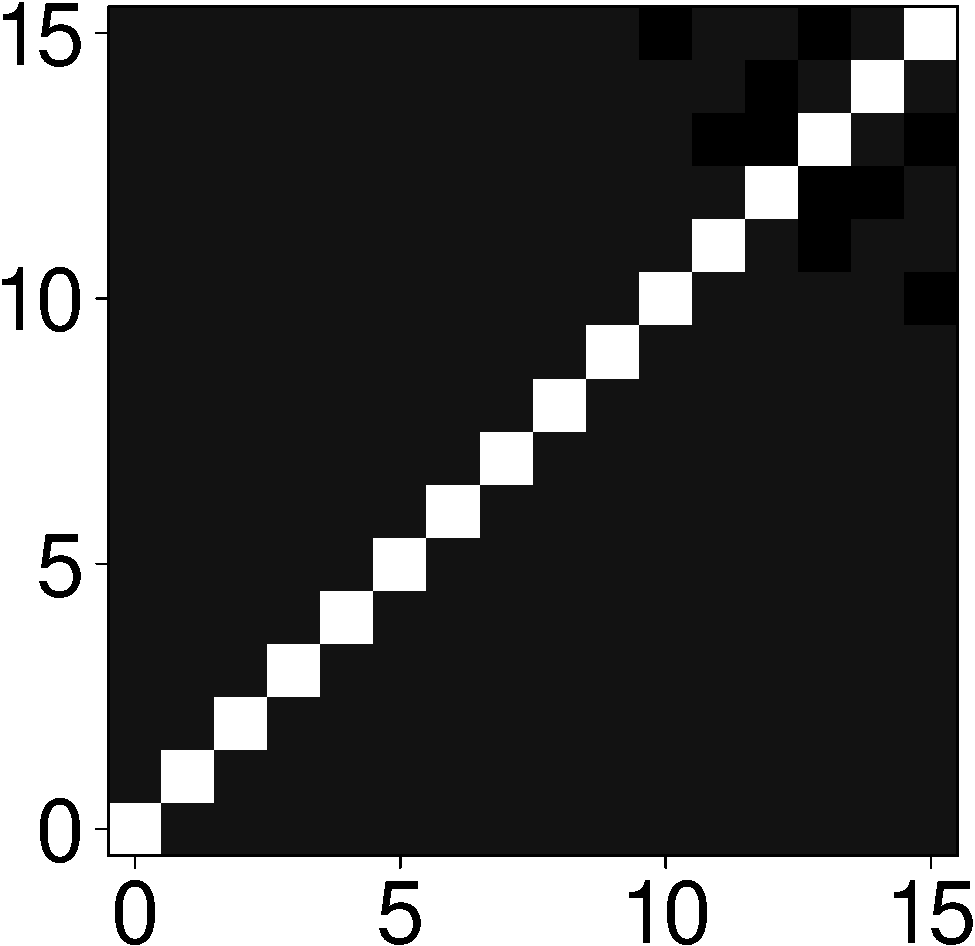
\includegraphics[width=\oneFPage\textwidth]{figures/mechanism/matrices/opteron/ssca2_16.pdf}
	}
	\subfigure[vacation]{
		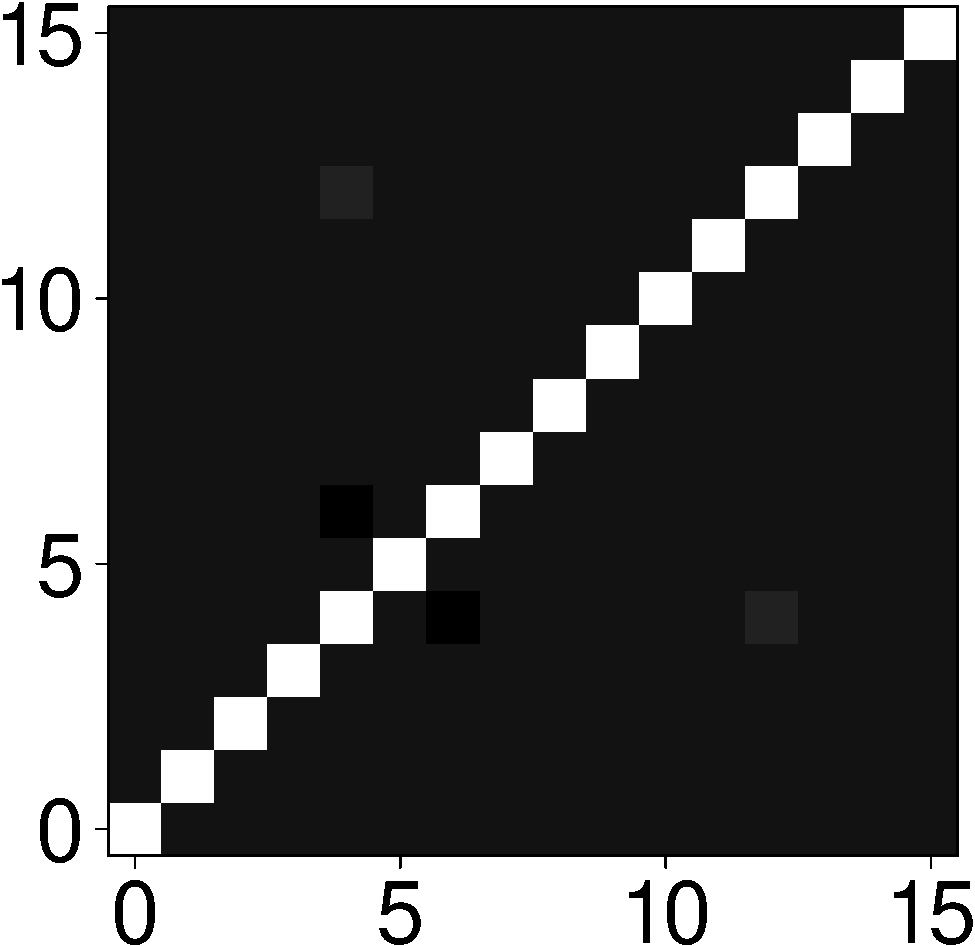
\includegraphics[width=\oneFPage\textwidth]{figures/mechanism/matrices/opteron/vacation_16.pdf}
	}
	\subfigure[yada]{
		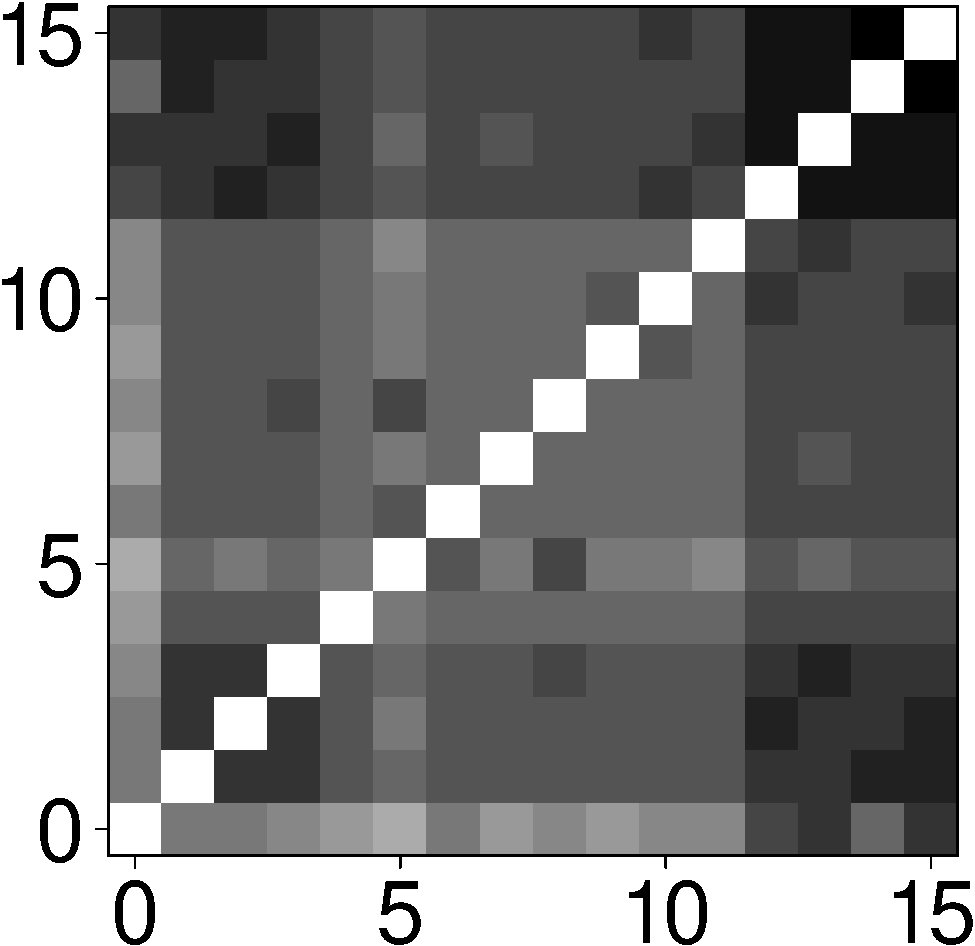
\includegraphics[width=\oneFPage\textwidth]{figures/mechanism/matrices/opteron/yada_16.pdf}
	}
	\subfigure[redblacktree]{
		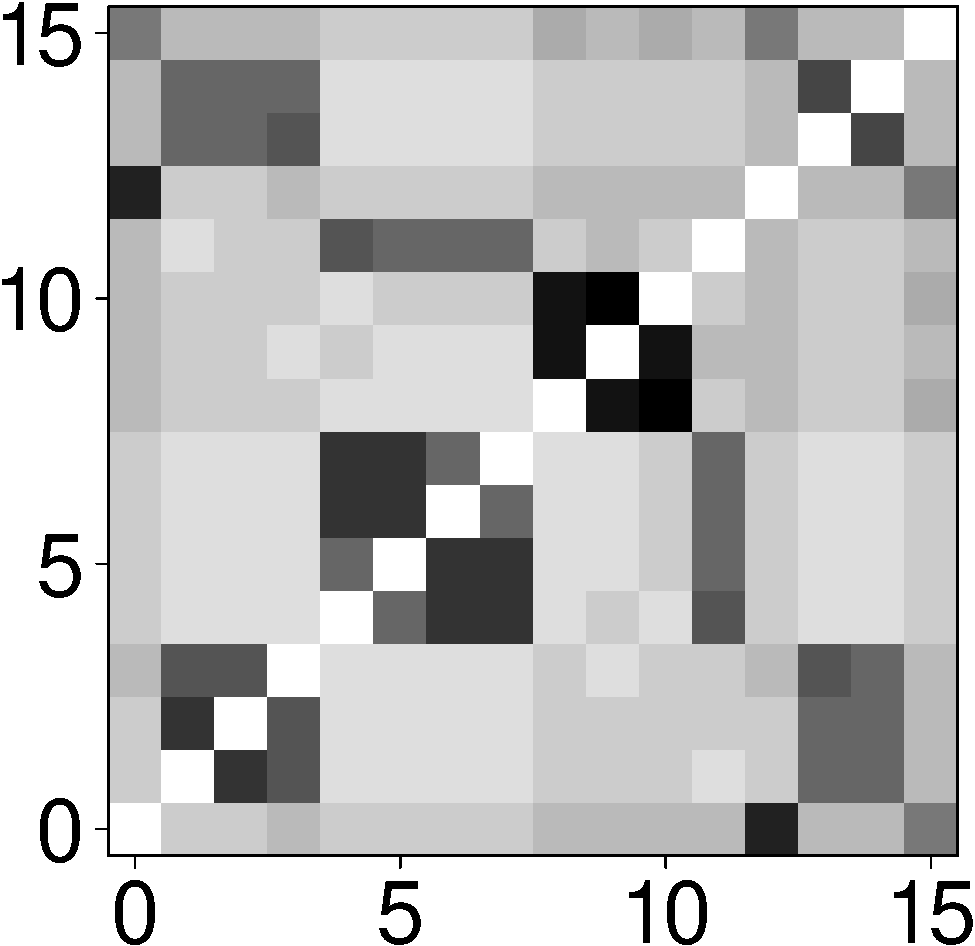
\includegraphics[width=\oneFPage\textwidth]{figures/mechanism/matrices/opteron/redblacktree_16.pdf}
	}
	\subfigure[hashmap]{
		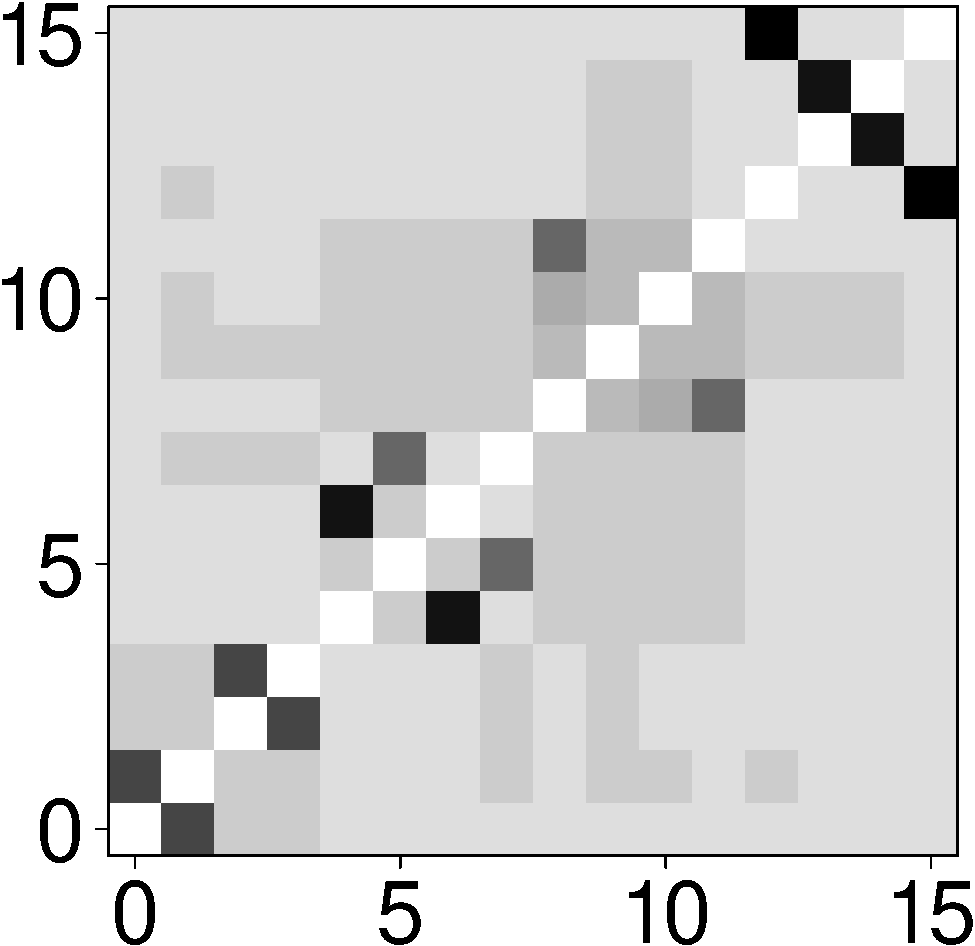
\includegraphics[width=\oneFPage\textwidth]{figures/mechanism/matrices/opteron/hashmap_16.pdf}
	}
	\caption{Communication matrices - 16 threads.}
	\label{fig:commMatrOpt16}
\end{figure}

\begin{figure}[!bt]
	\centering
	\subfigure[bayes]{
		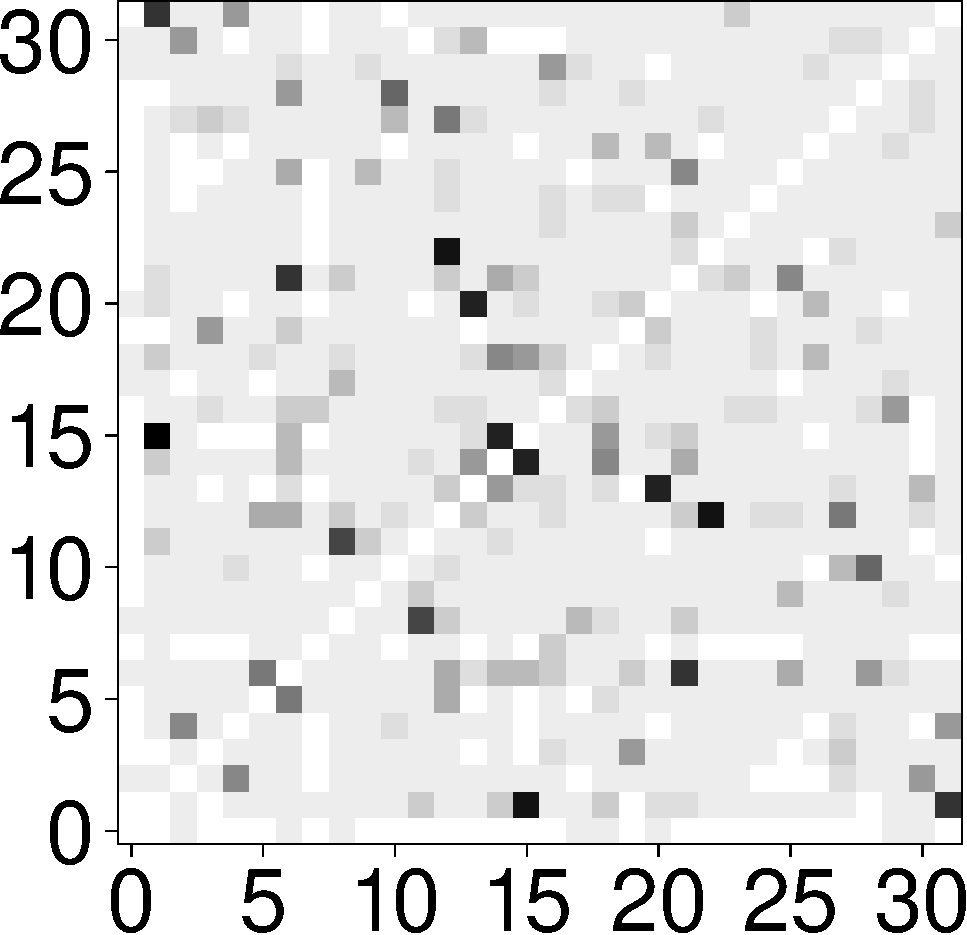
\includegraphics[width=\oneFPage\textwidth]{figures/mechanism/matrices/xeon/bayes_32.pdf}
	}
	\subfigure[genome]{
		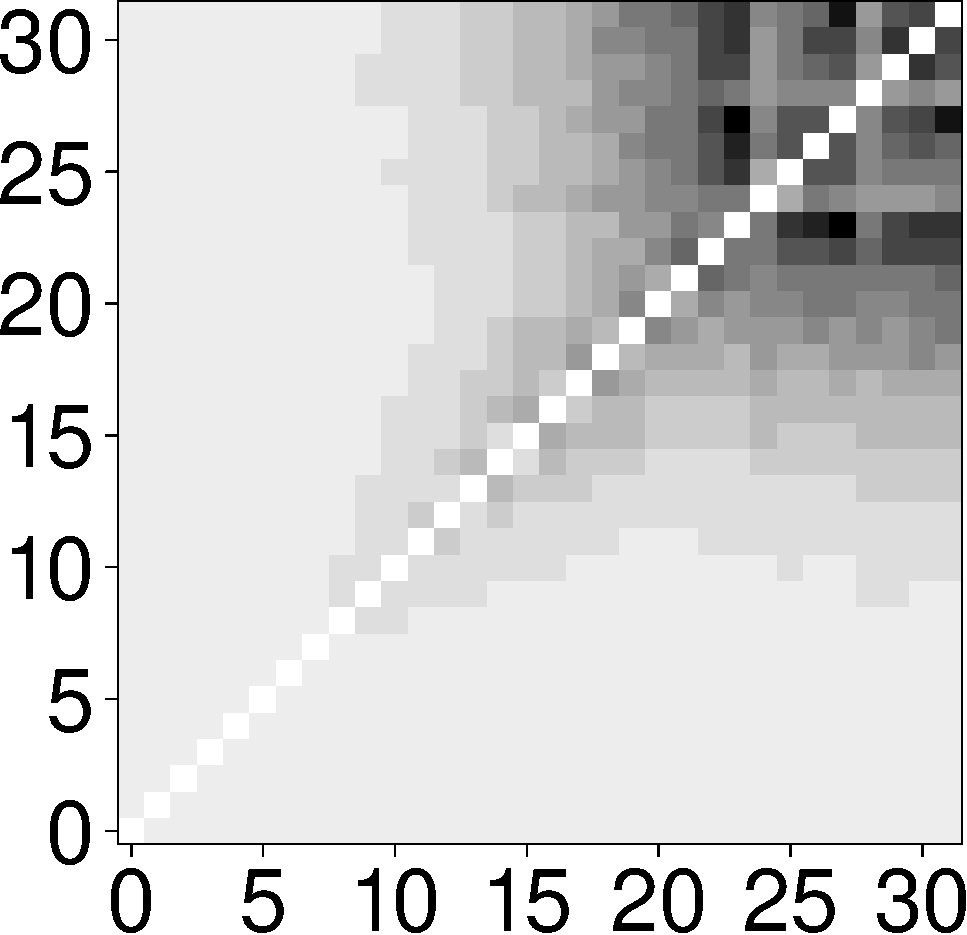
\includegraphics[width=\oneFPage\textwidth]{figures/mechanism/matrices/xeon/genome_32.pdf}
	}
	\subfigure[intruder]{
		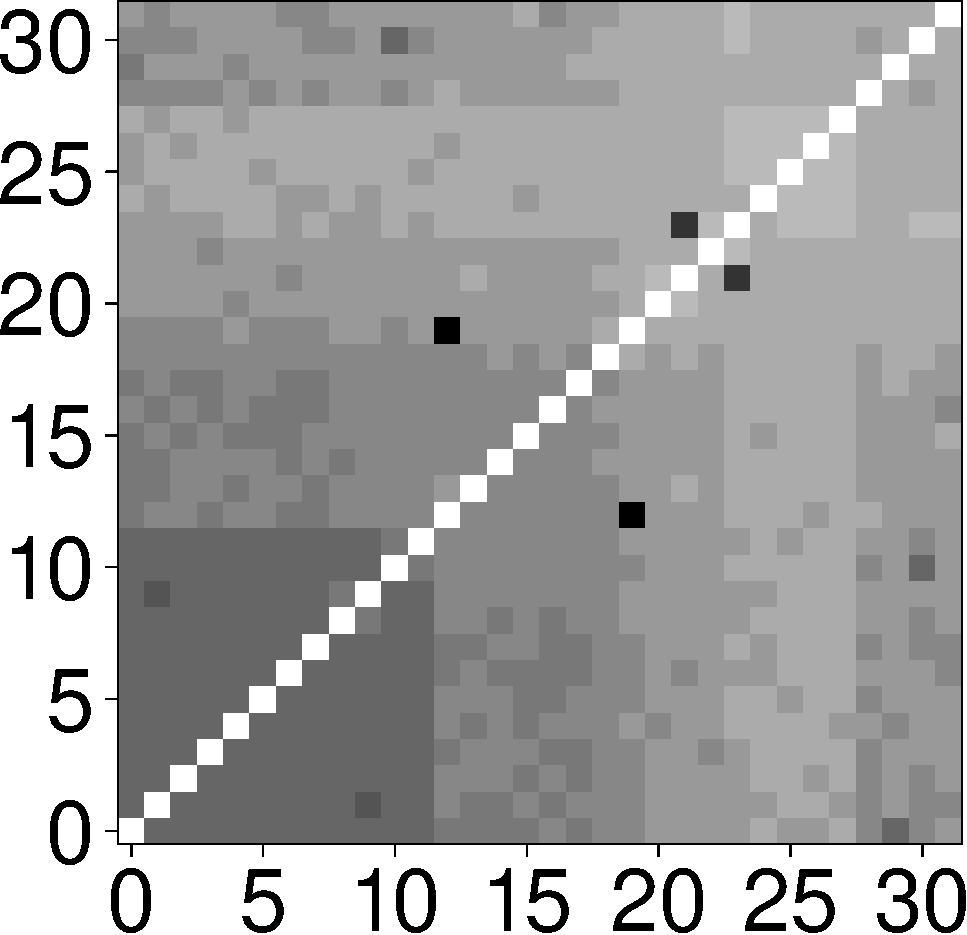
\includegraphics[width=\oneFPage\textwidth]{figures/mechanism/matrices/xeon/intruder_32.pdf}
	}
	\subfigure[kmeans]{
		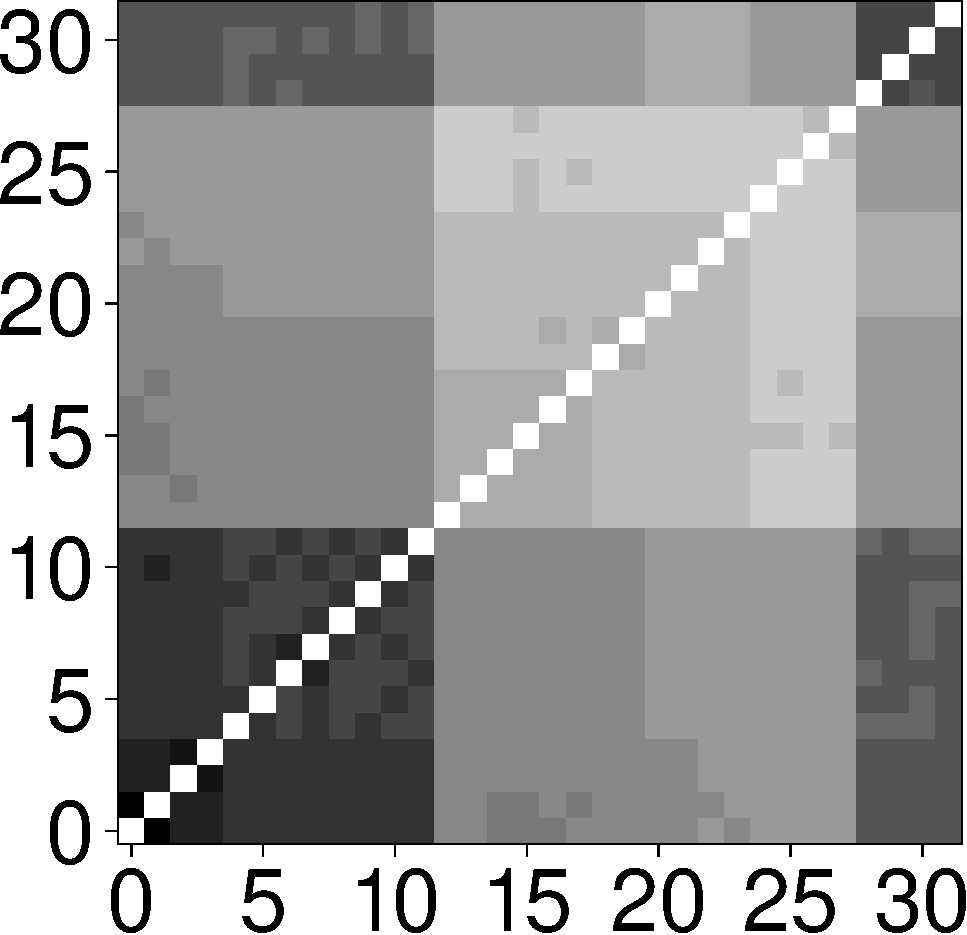
\includegraphics[width=\oneFPage\textwidth]{figures/mechanism/matrices/xeon/kmeans_32.pdf}
	}
	\subfigure[labyrinth]{
		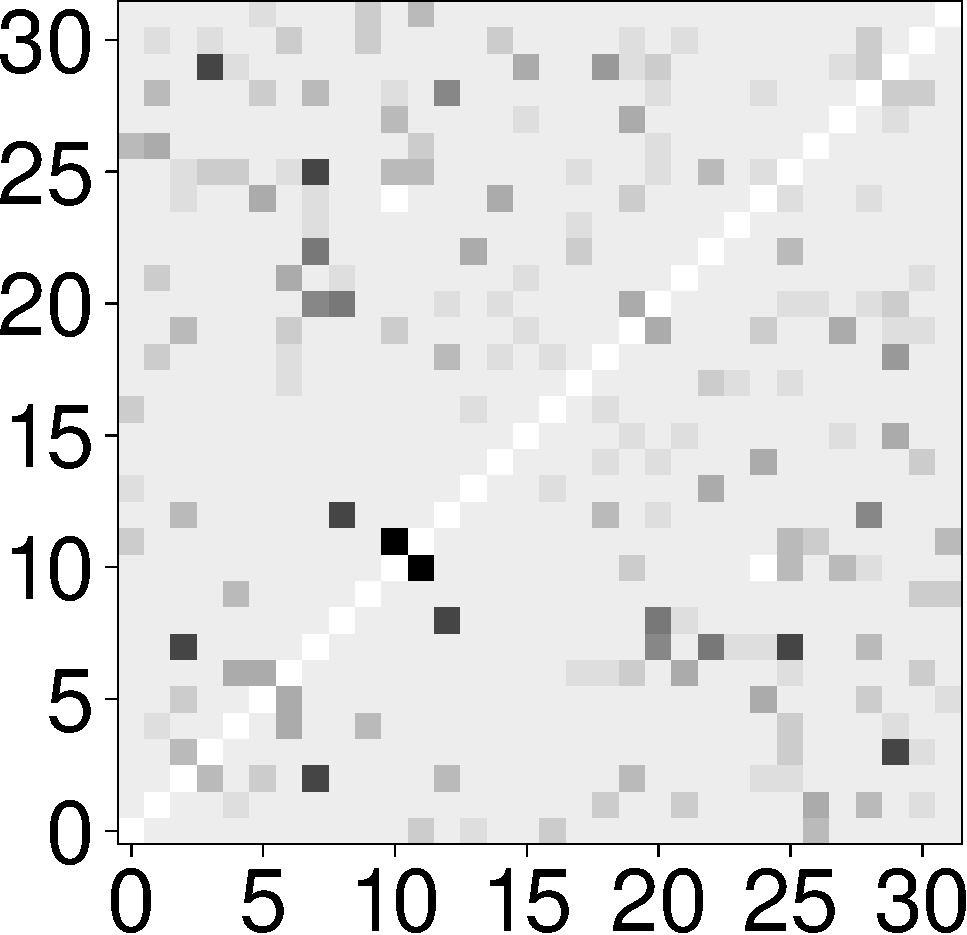
\includegraphics[width=\oneFPage\textwidth]{figures/mechanism/matrices/xeon/labyrinth_32.pdf}
	}
\\
	\subfigure[ssca2]{
		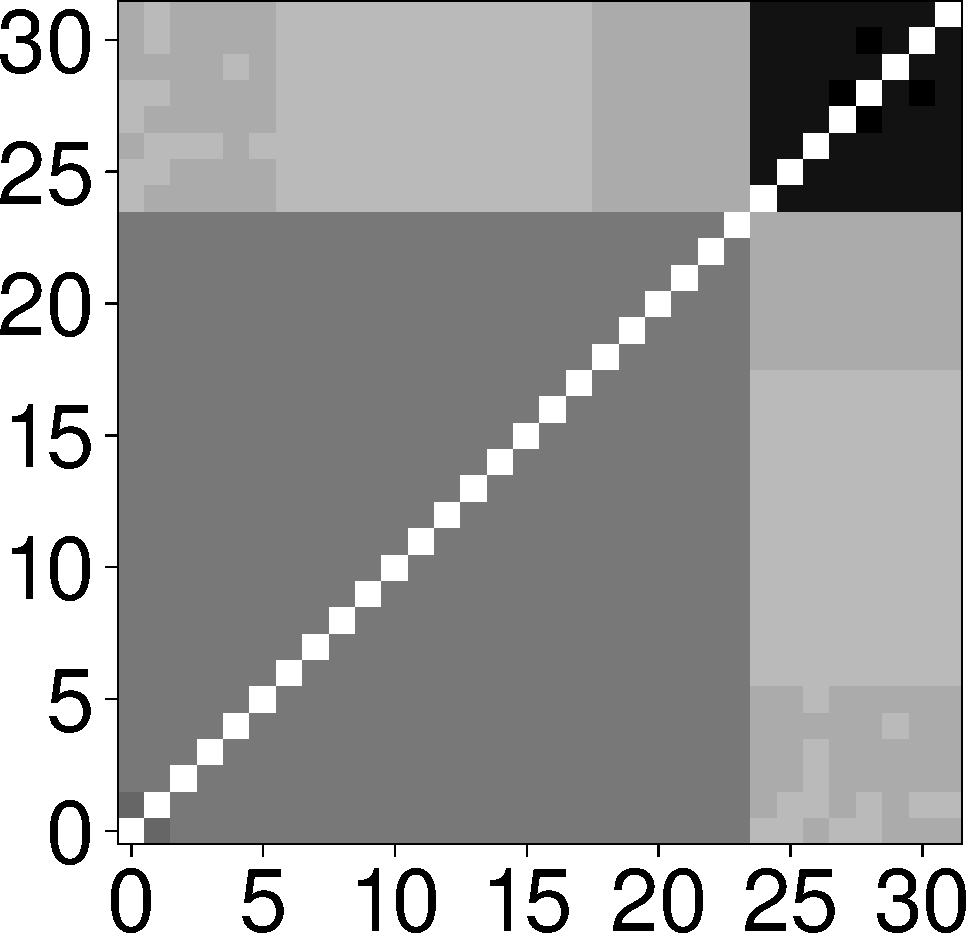
\includegraphics[width=\oneFPage\textwidth]{figures/mechanism/matrices/xeon/ssca2_32.pdf}
	}
	\subfigure[vacation]{
		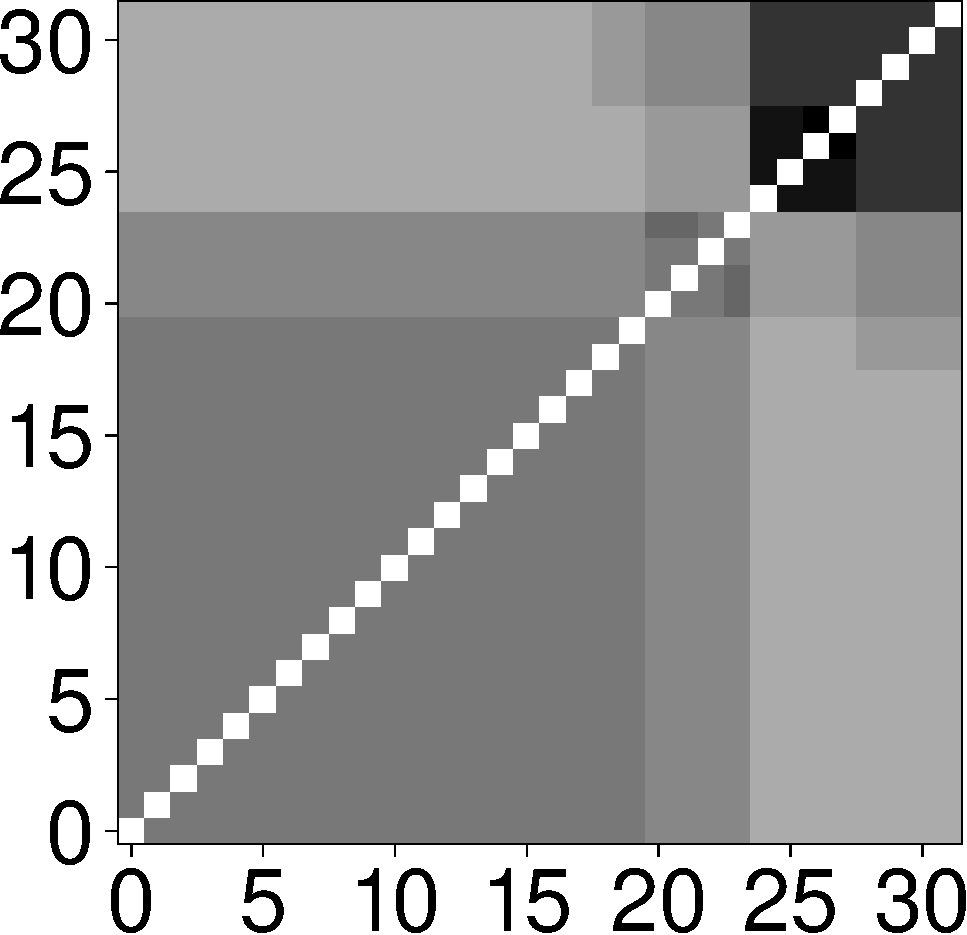
\includegraphics[width=\oneFPage\textwidth]{figures/mechanism/matrices/xeon/vacation_32.pdf}
	}
	\subfigure[yada]{
		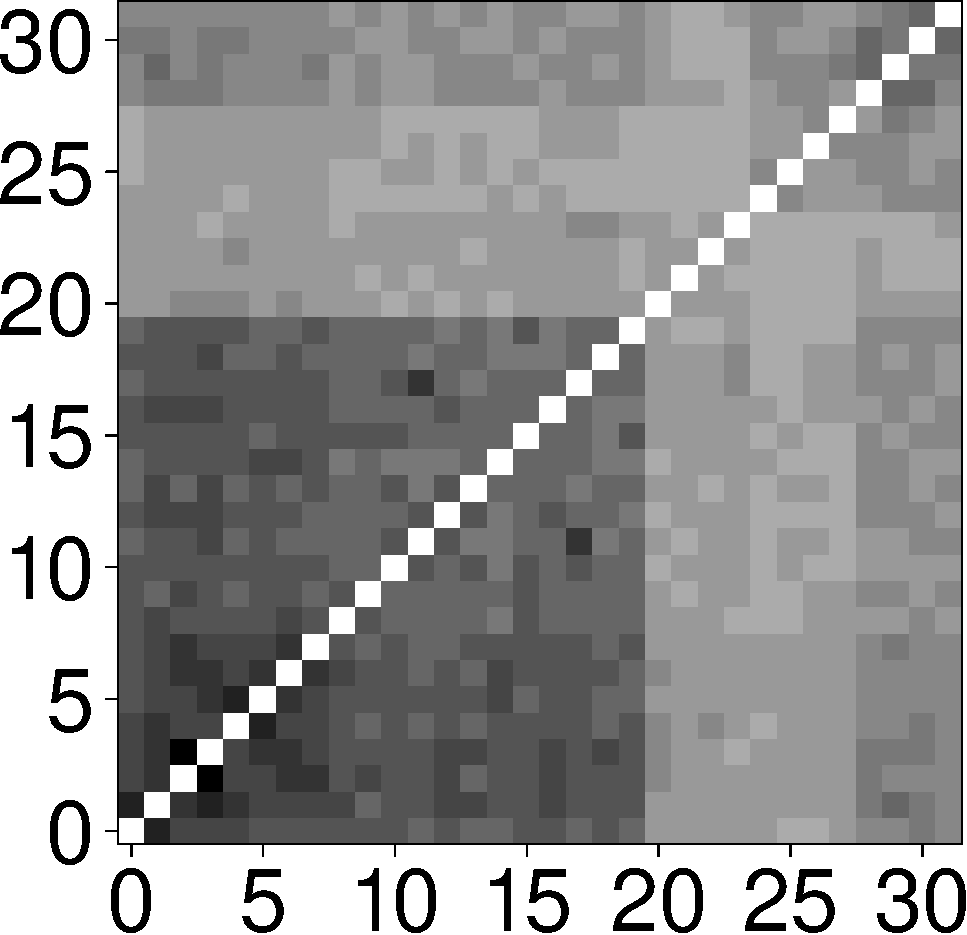
\includegraphics[width=\oneFPage\textwidth]{figures/mechanism/matrices/xeon/yada_32.pdf}
	}
	\subfigure[redblacktree]{
		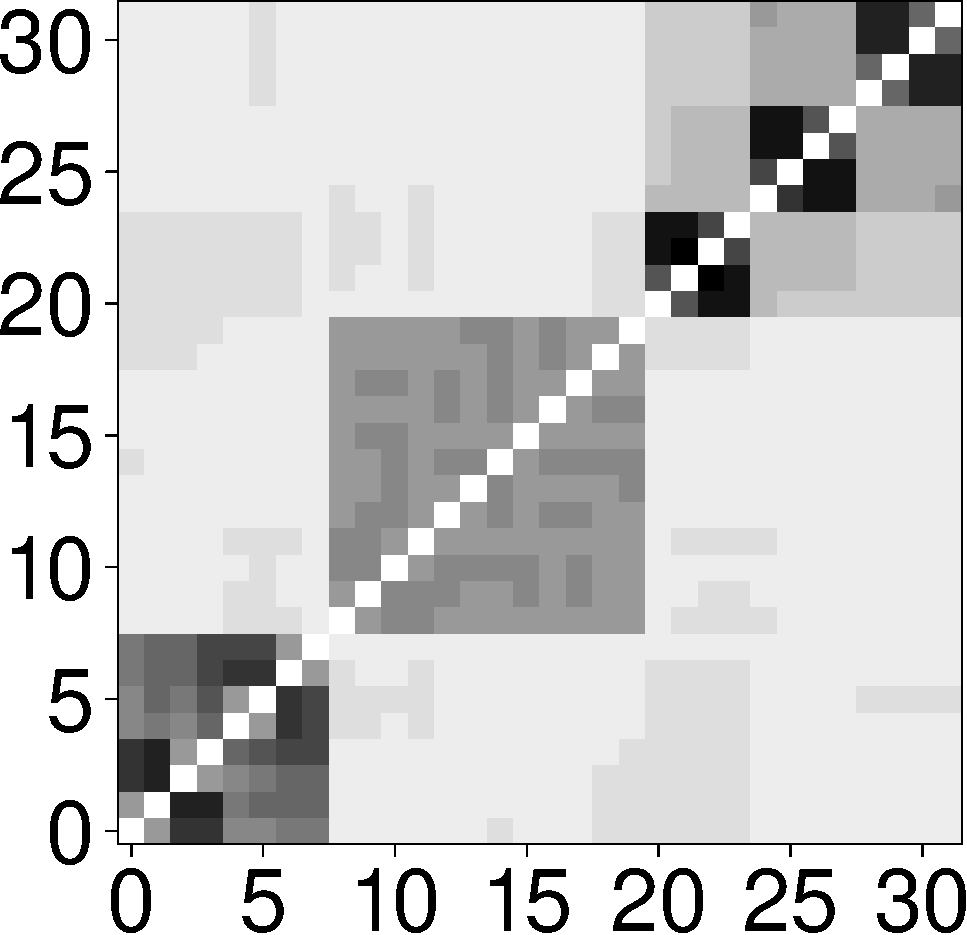
\includegraphics[width=\oneFPage\textwidth]{figures/mechanism/matrices/xeon/redblacktree_32.pdf}
	}
	\subfigure[hashmap]{
		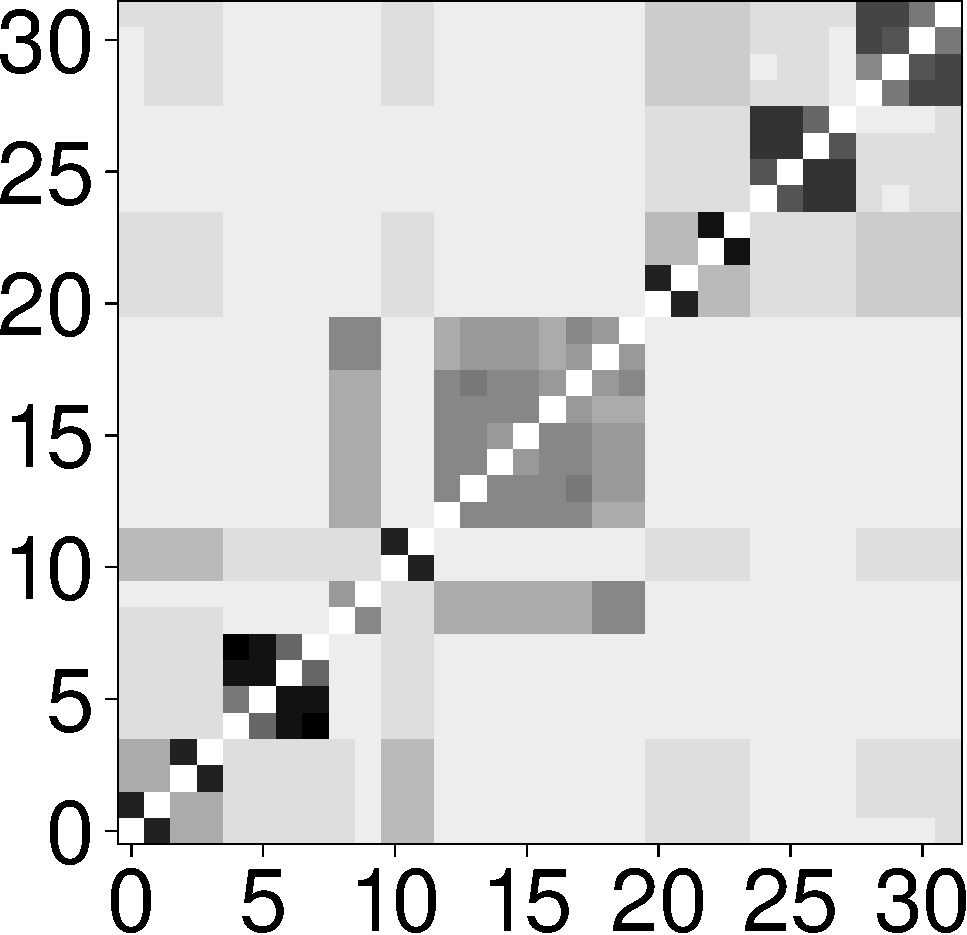
\includegraphics[width=\oneFPage\textwidth]{figures/mechanism/matrices/xeon/hashmap_32.pdf}
	}
	\caption{Communication matrices - 32 threads.}
\end{figure}

%%%%%%%%%%%%%%%%%%%

\begin{figure}[!bt]
	\centering
	\subfigure[bayes]{
		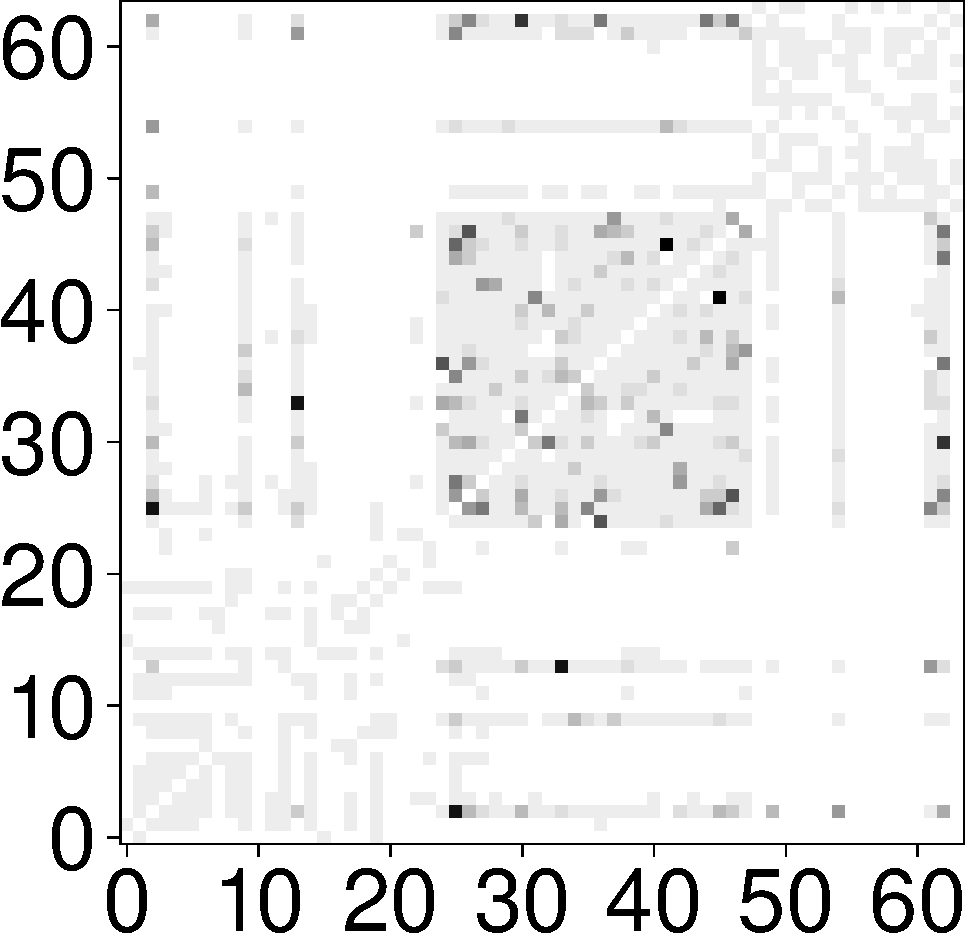
\includegraphics[width=\oneFPage\textwidth]{figures/mechanism/matrices/xeon/bayes_64.pdf}
	}
	\subfigure[genome]{
		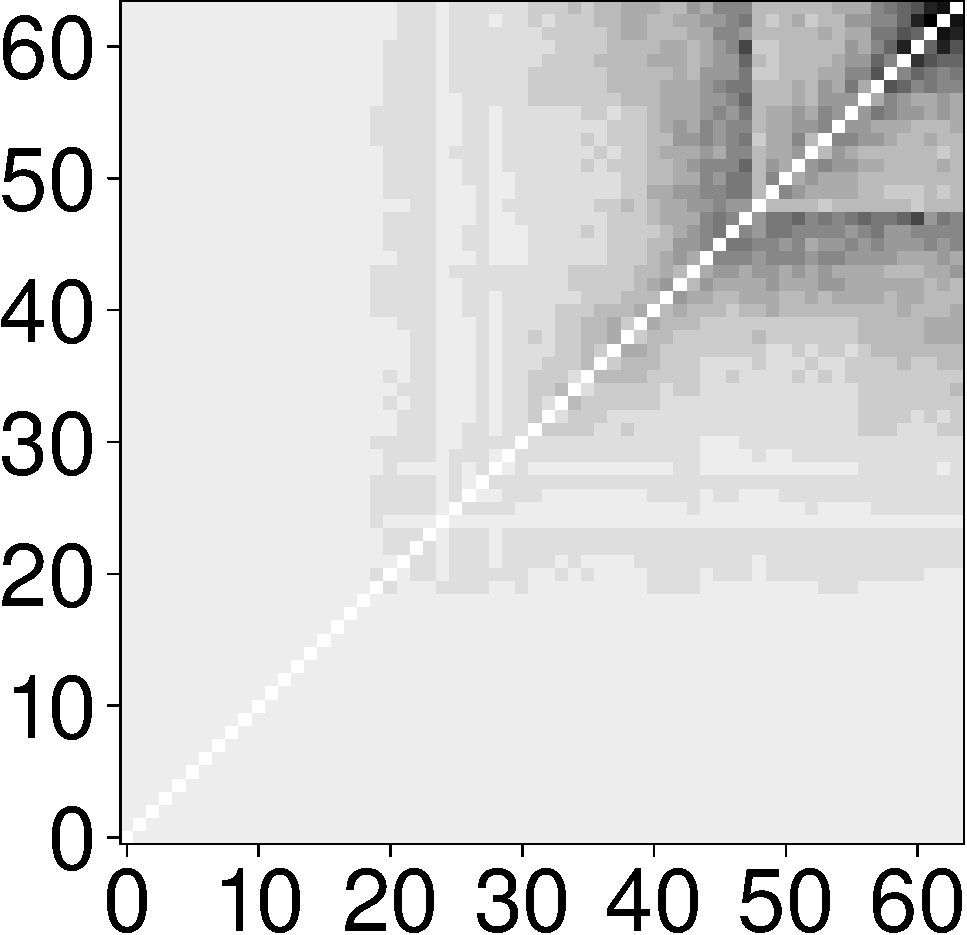
\includegraphics[width=\oneFPage\textwidth]{figures/mechanism/matrices/xeon/genome_64.pdf}
	}
	\subfigure[intruder]{
		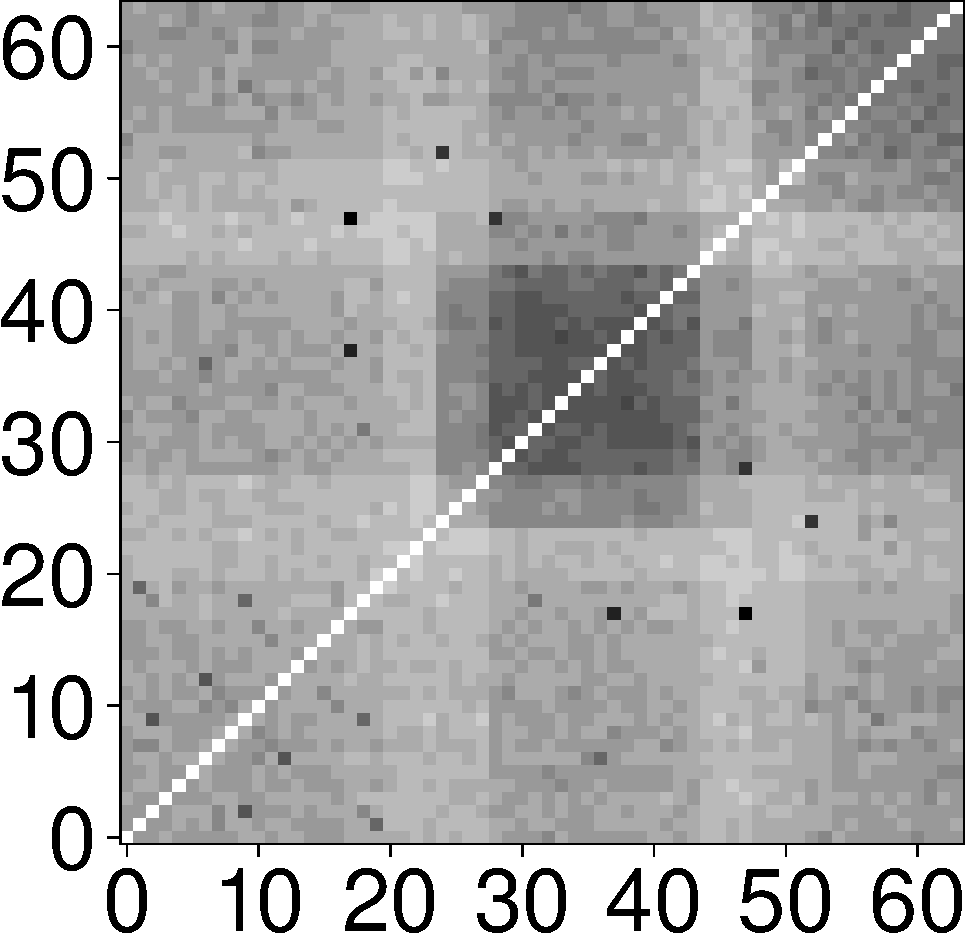
\includegraphics[width=\oneFPage\textwidth]{figures/mechanism/matrices/xeon/intruder_64.pdf}
	}
	\subfigure[kmeans]{
		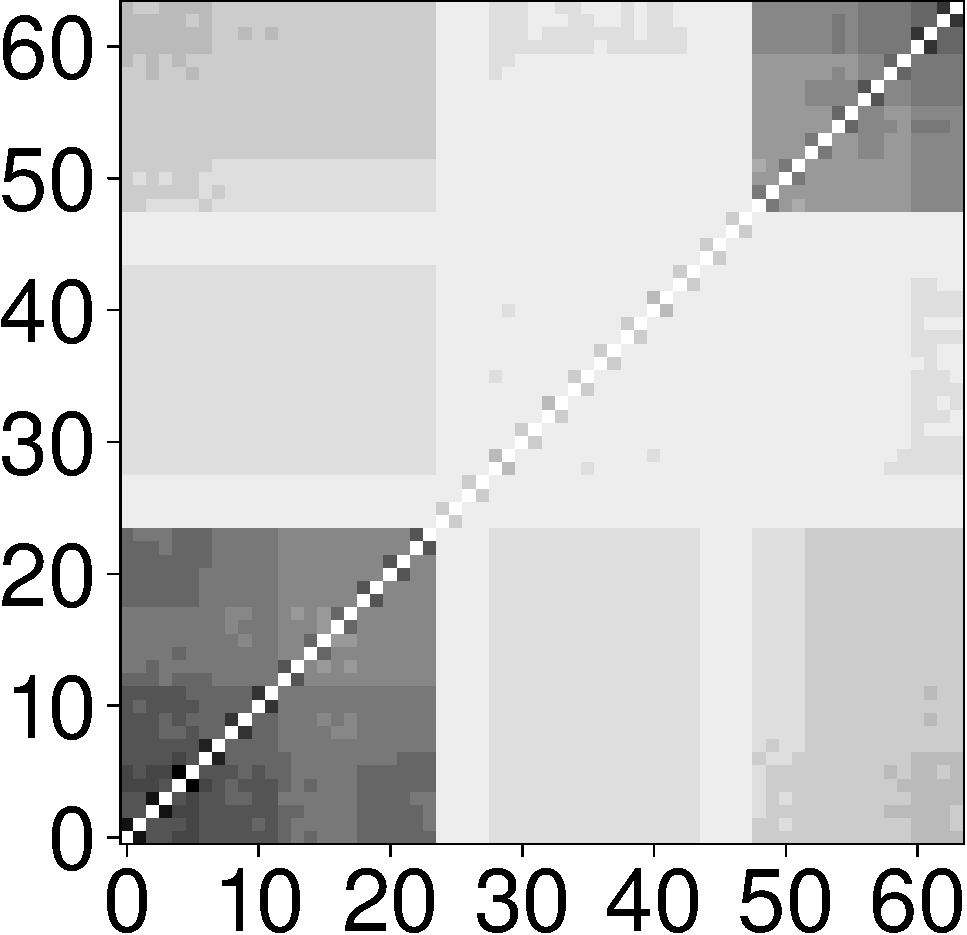
\includegraphics[width=\oneFPage\textwidth]{figures/mechanism/matrices/xeon/kmeans_64.pdf}
	}
	\subfigure[labyrinth]{
		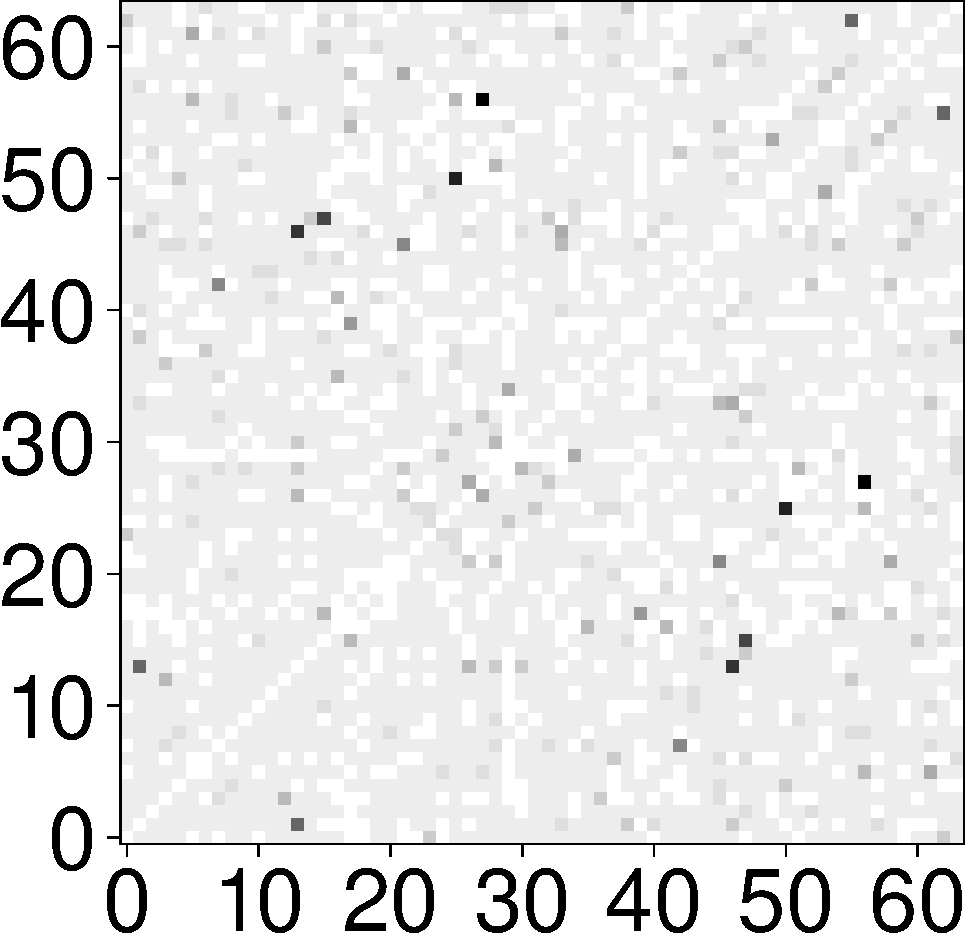
\includegraphics[width=\oneFPage\textwidth]{figures/mechanism/matrices/xeon/labyrinth_64.pdf}
	}
	\\
	\subfigure[ssca2]{
		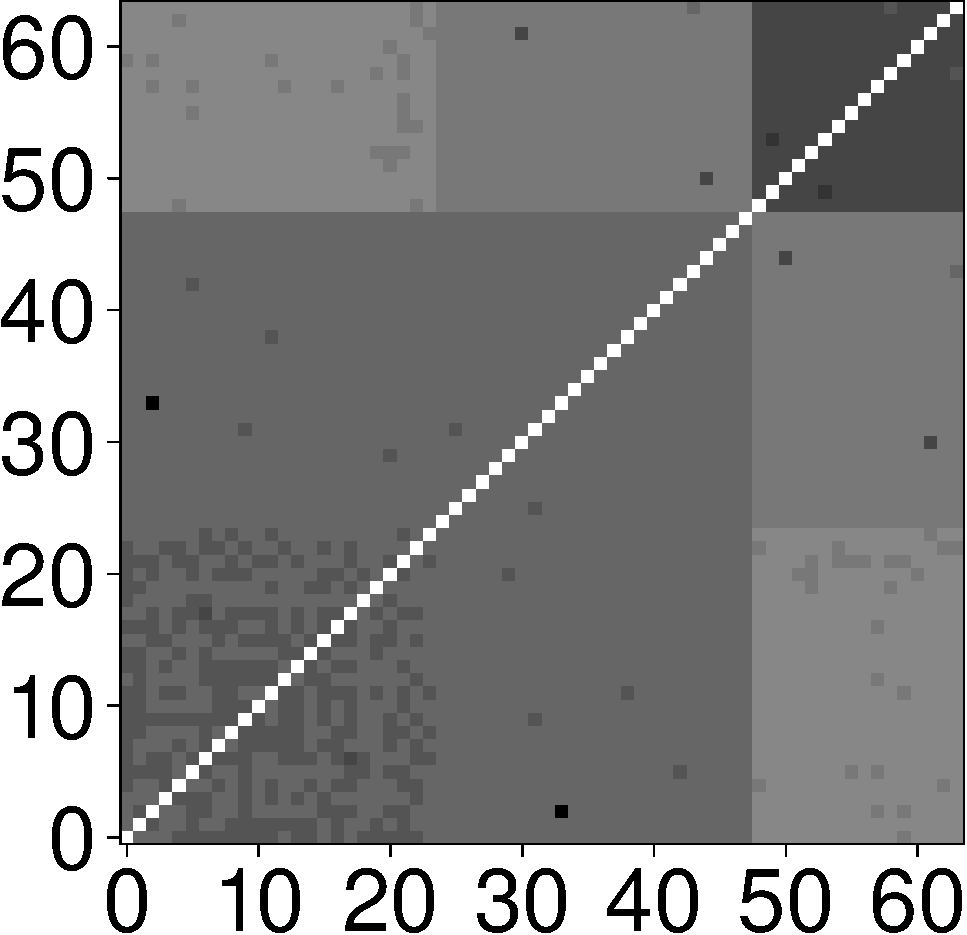
\includegraphics[width=\oneFPage\textwidth]{figures/mechanism/matrices/xeon/ssca2_64.pdf}
	}
	\subfigure[vacation]{
		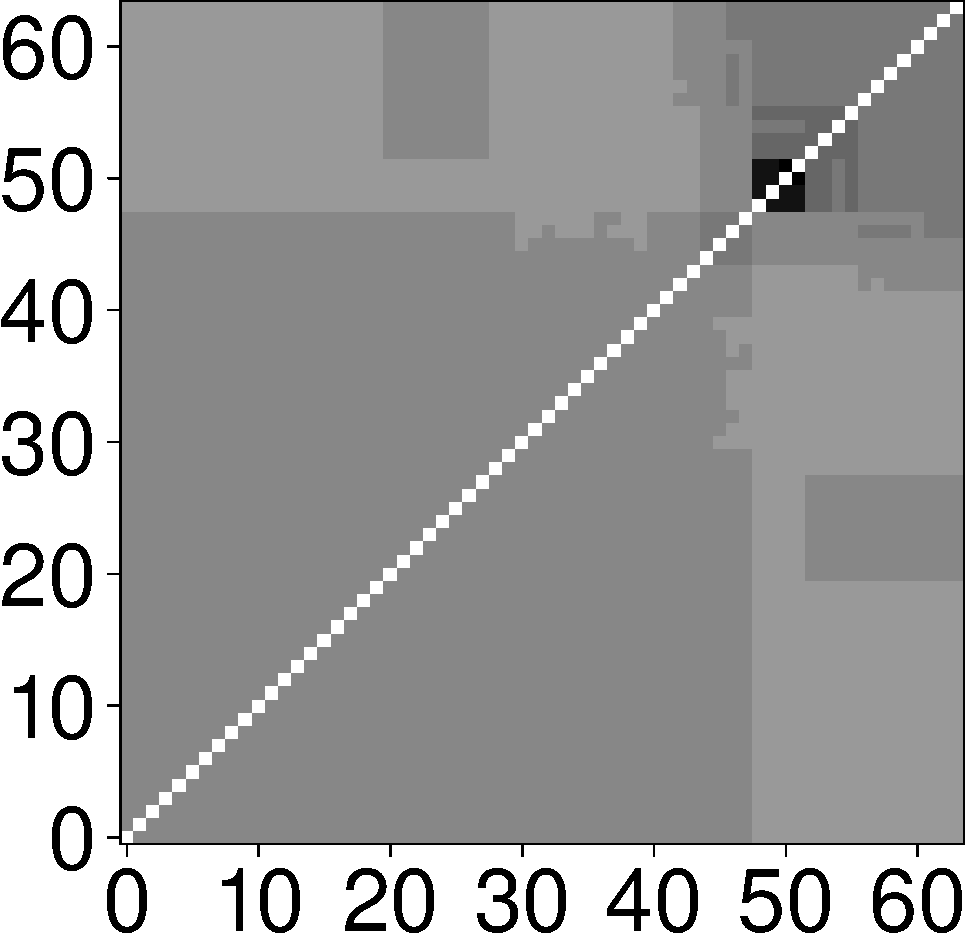
\includegraphics[width=\oneFPage\textwidth]{figures/mechanism/matrices/xeon/vacation_64.pdf}
	}
	\subfigure[yada]{
		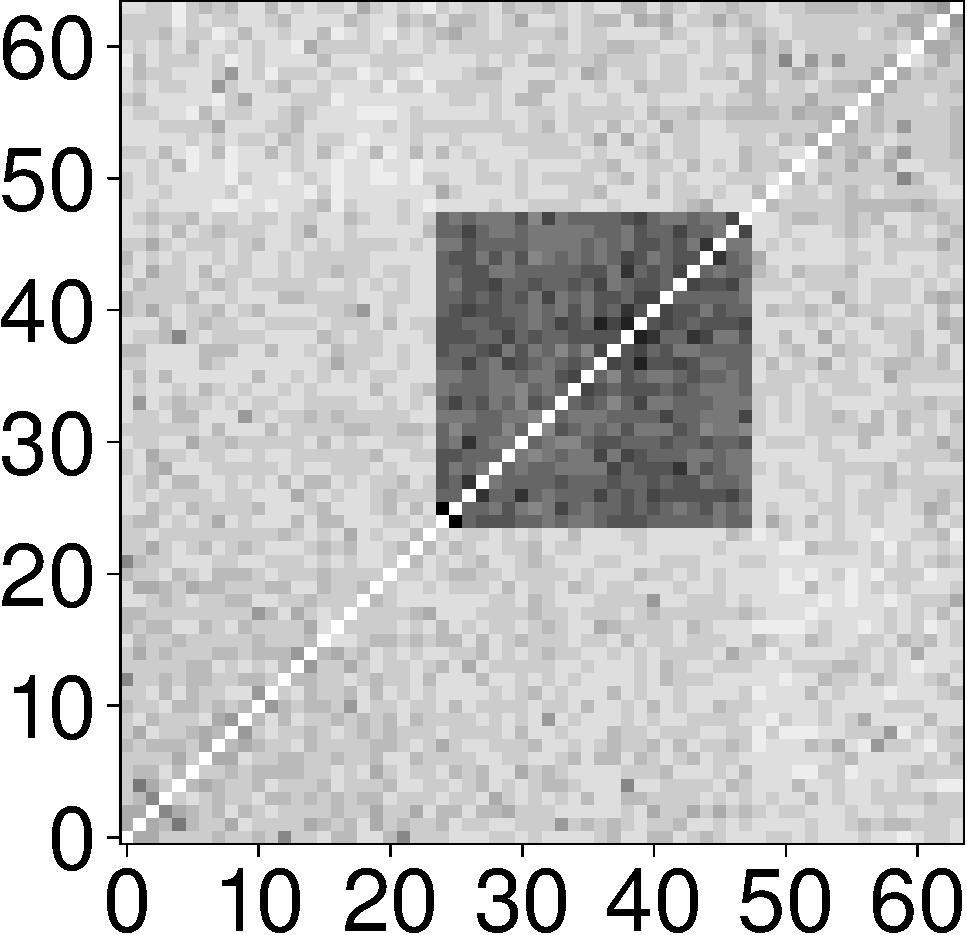
\includegraphics[width=\oneFPage\textwidth]{figures/mechanism/matrices/xeon/yada_64.pdf}
	}
	\subfigure[redblacktree]{
		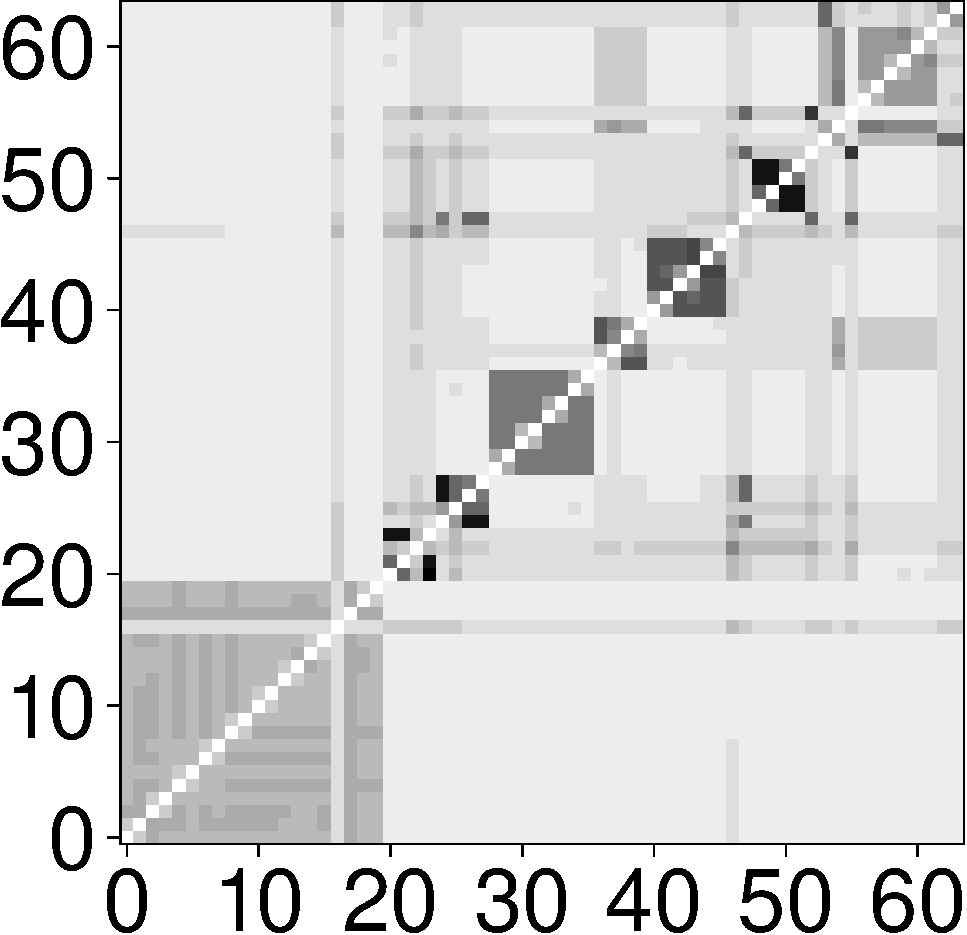
\includegraphics[width=\oneFPage\textwidth]{figures/mechanism/matrices/xeon/redblacktree_64.pdf}
	}
	\subfigure[hashmap]{
		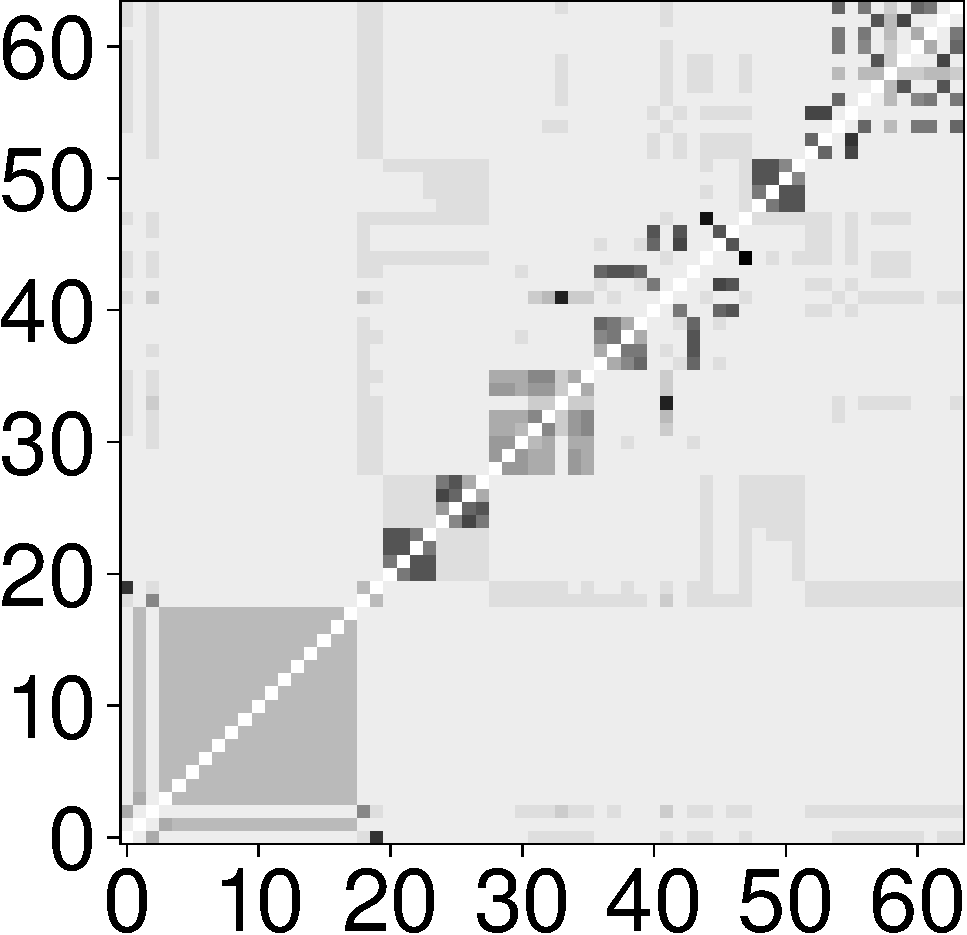
\includegraphics[width=\oneFPage\textwidth]{figures/mechanism/matrices/xeon/hashmap_64.pdf}
	}
	\caption{Communication matrices - 64 threads.}
\end{figure}

\begin{figure}[!tb]
	\centering
	\subfigure[bayes]{
		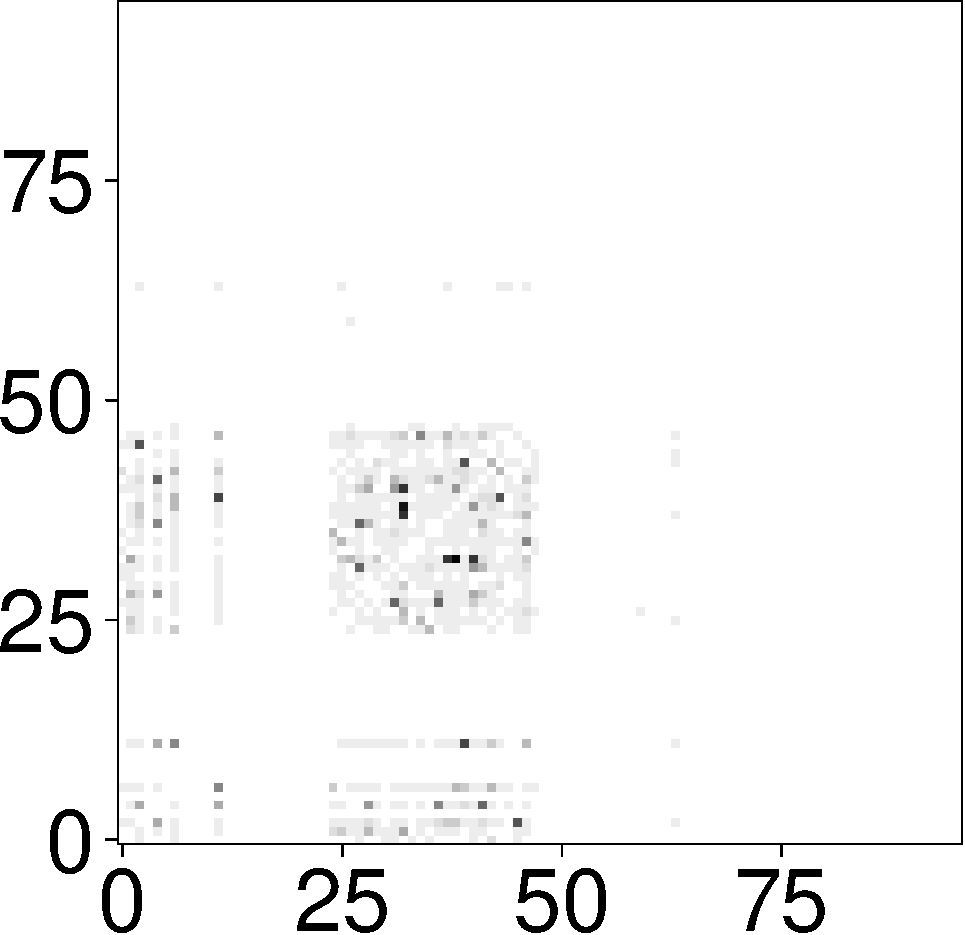
\includegraphics[width=\oneFPage\textwidth]{figures/mechanism/matrices/xeon/bayes_96.pdf}
	}
	\subfigure[genome]{
		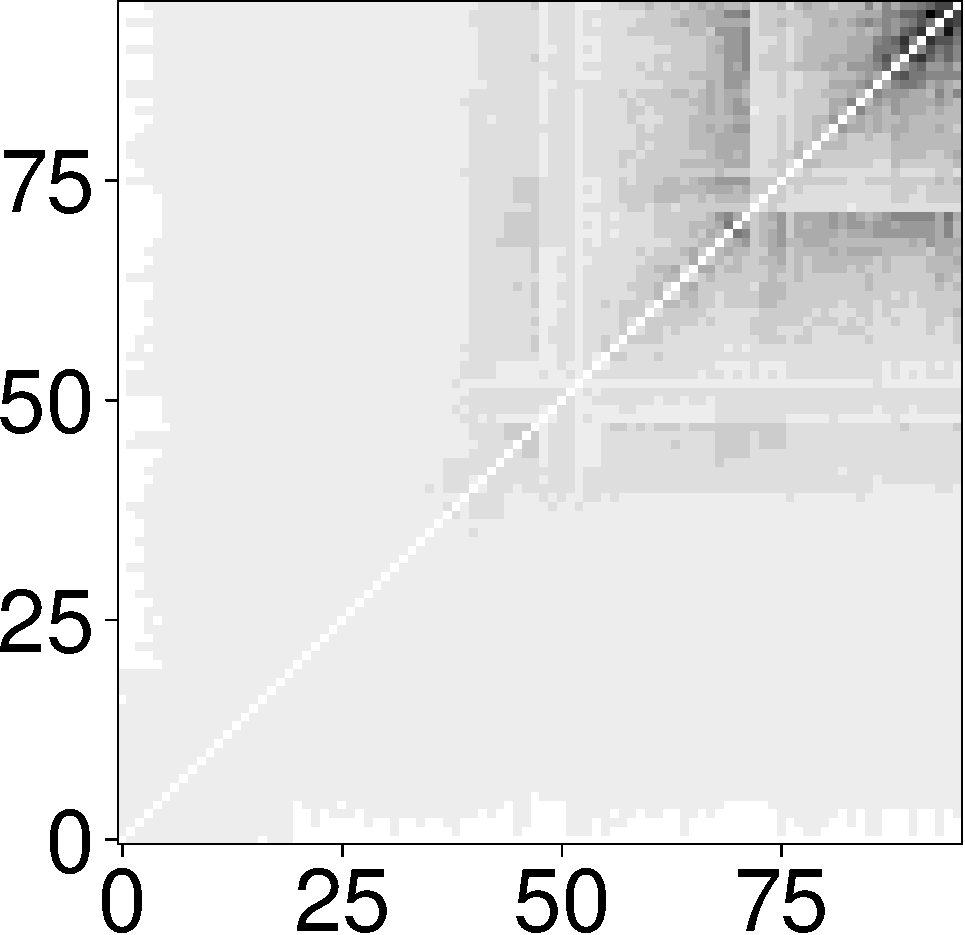
\includegraphics[width=\oneFPage\textwidth]{figures/mechanism/matrices/xeon/genome_96.pdf}
	}
	\subfigure[intruder]{
		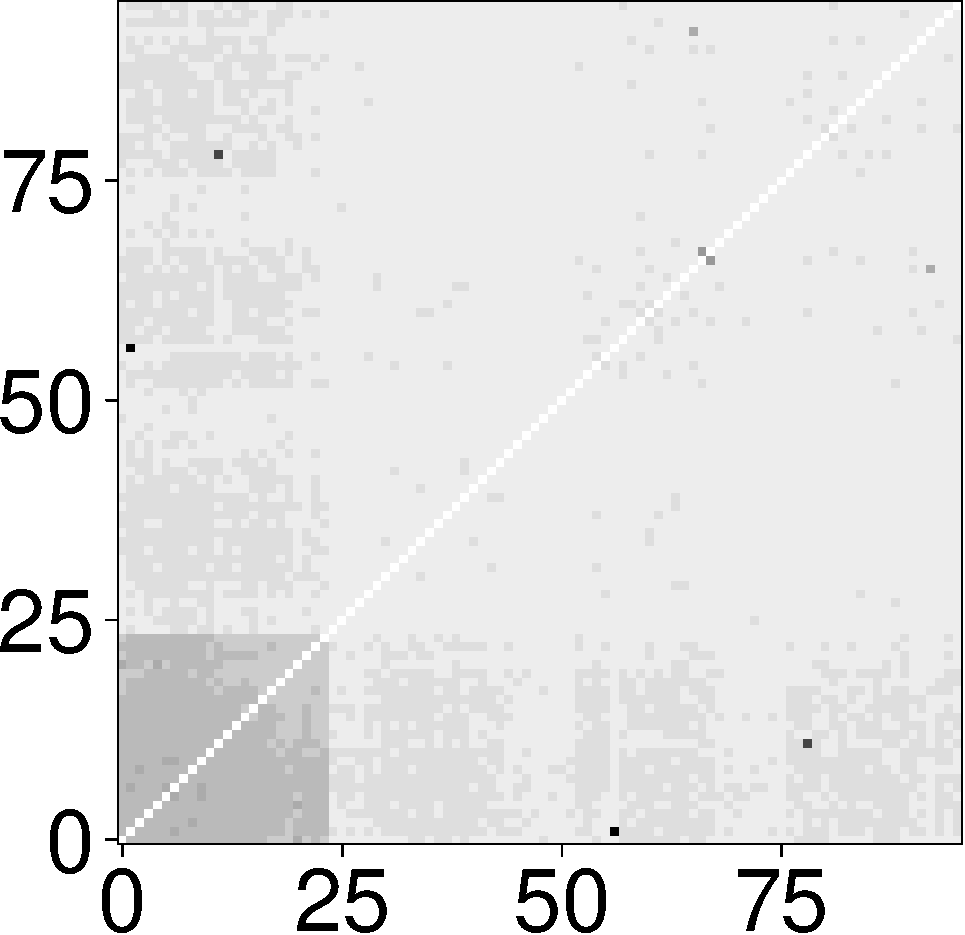
\includegraphics[width=\oneFPage\textwidth]{figures/mechanism/matrices/xeon/intruder_96.pdf}
	}
	\subfigure[kmeans]{
		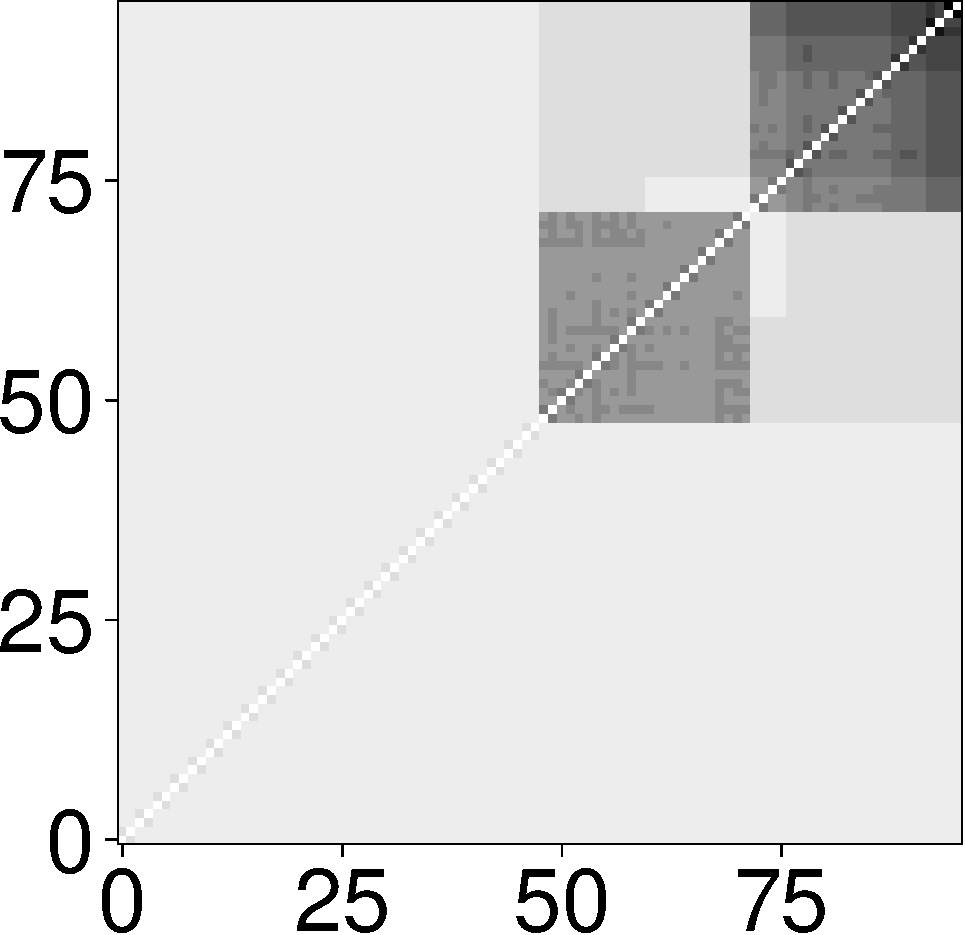
\includegraphics[width=\oneFPage\textwidth]{figures/mechanism/matrices/xeon/kmeans_96.pdf}
	}
	\subfigure[labyrinth]{
		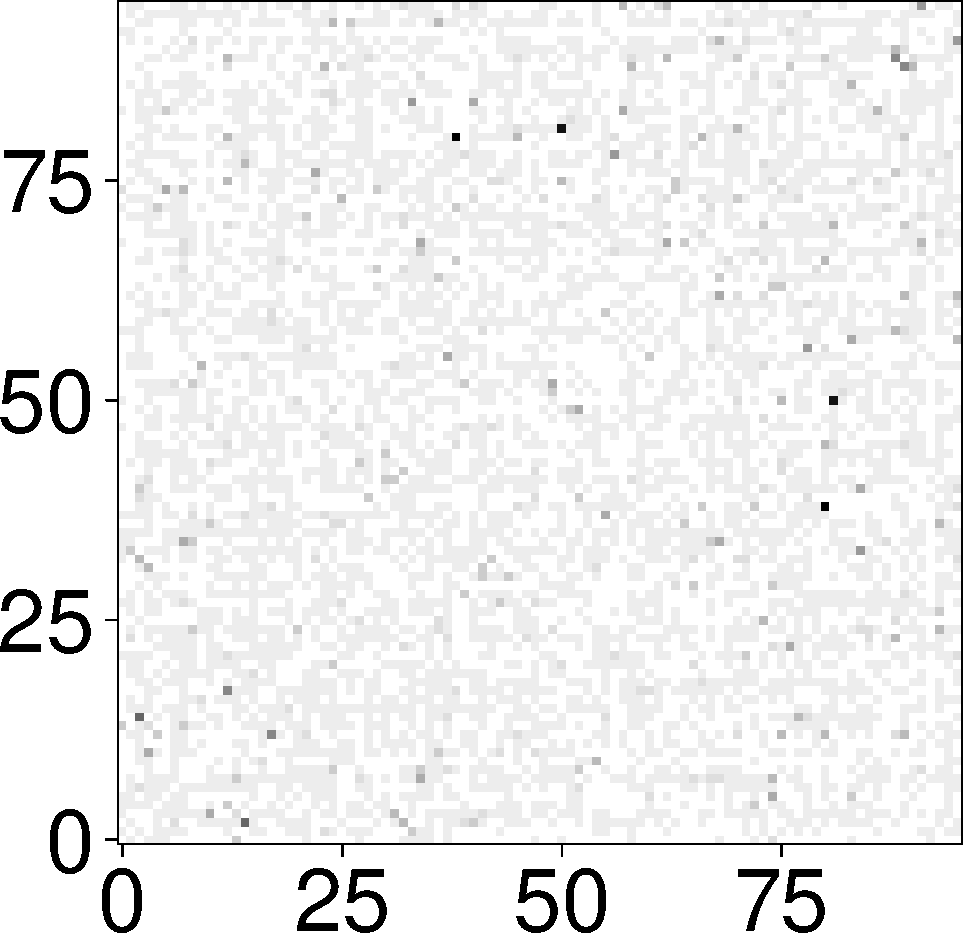
\includegraphics[width=\oneFPage\textwidth]{figures/mechanism/matrices/xeon/labyrinth_96.pdf}
	}
	\\
	\subfigure[ssca2]{
		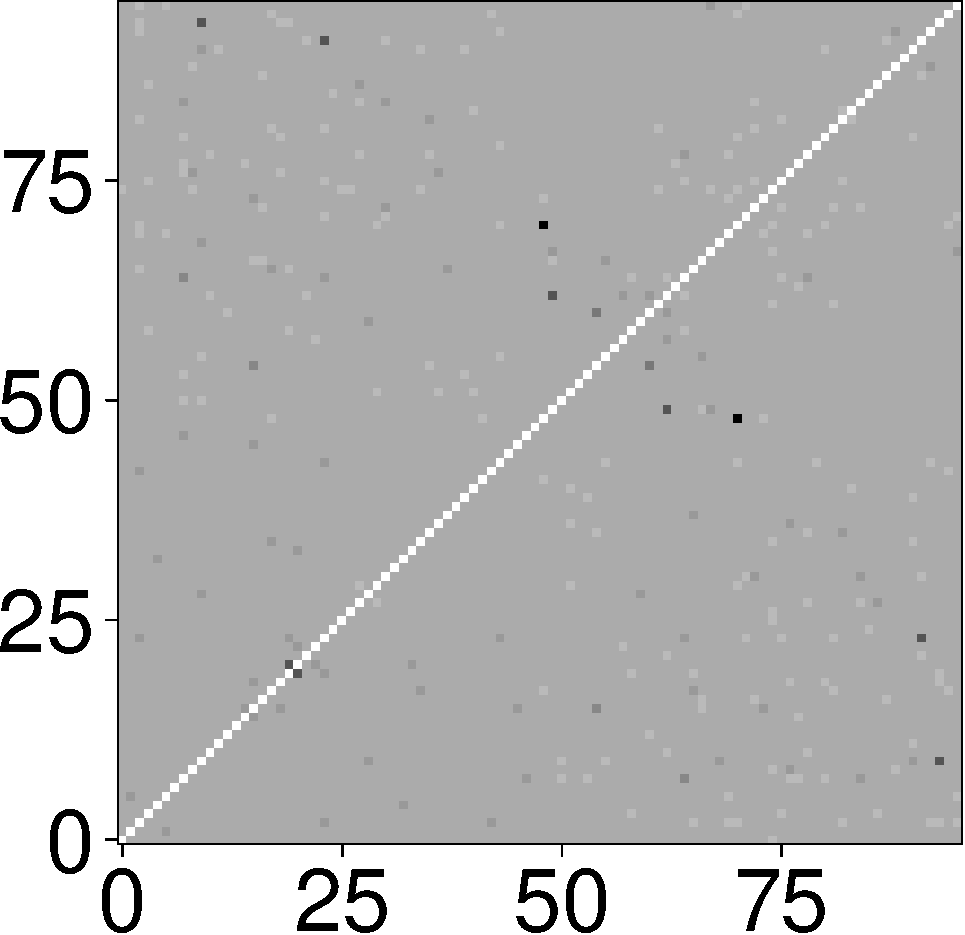
\includegraphics[width=\oneFPage\textwidth]{figures/mechanism/matrices/xeon/ssca2_96.pdf}
	}
	\subfigure[vacation]{
		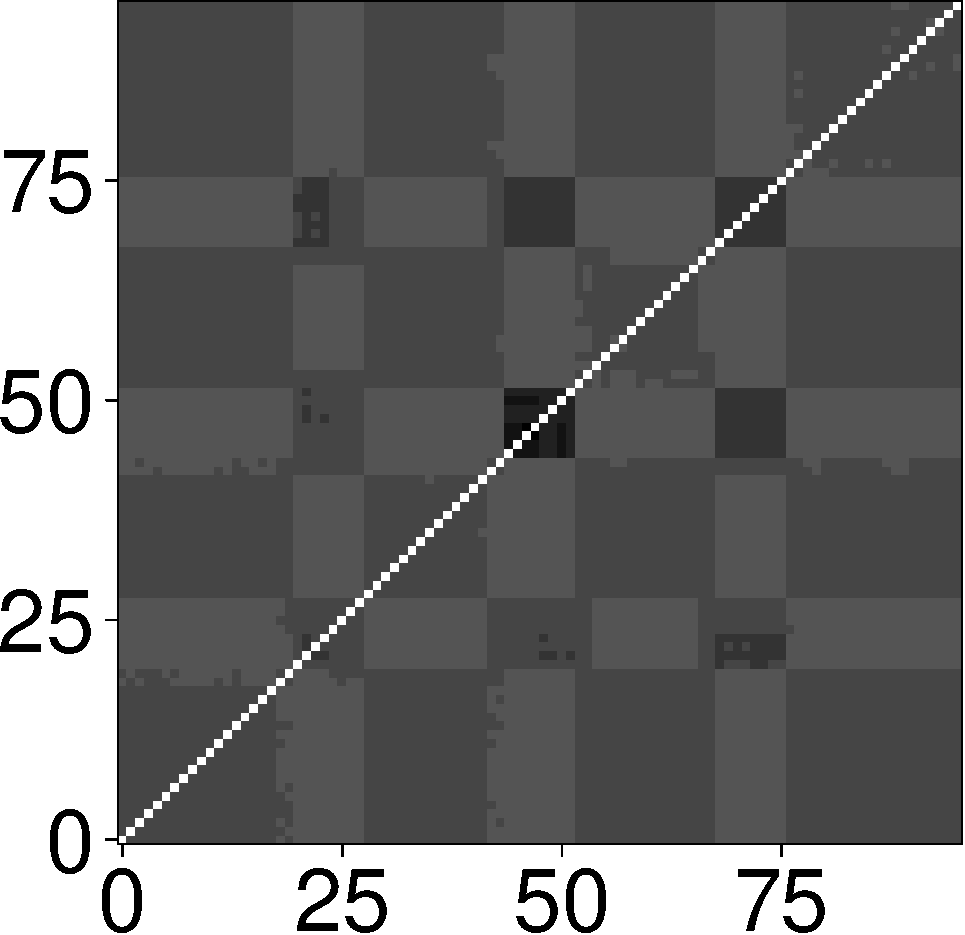
\includegraphics[width=\oneFPage\textwidth]{figures/mechanism/matrices/xeon/vacation_96.pdf}
	}
	\subfigure[yada]{
		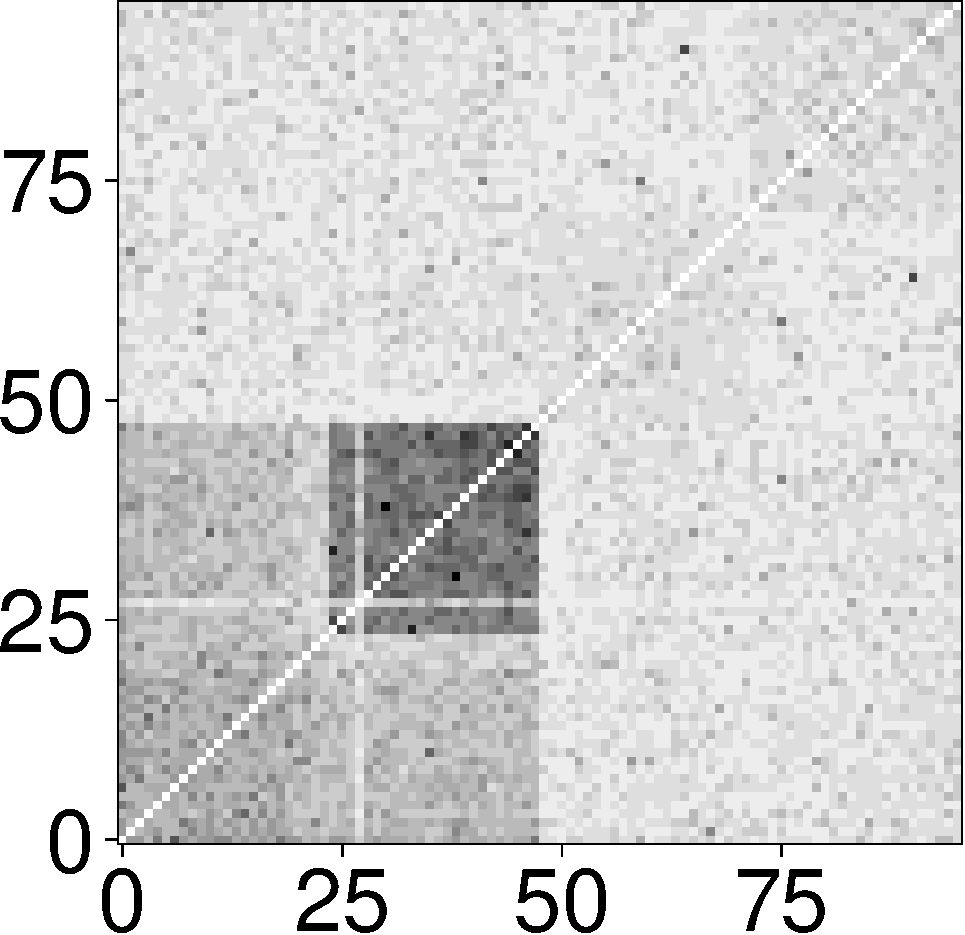
\includegraphics[width=\oneFPage\textwidth]{figures/mechanism/matrices/xeon/yada_96.pdf}
	}
	\subfigure[redblacktree]{
		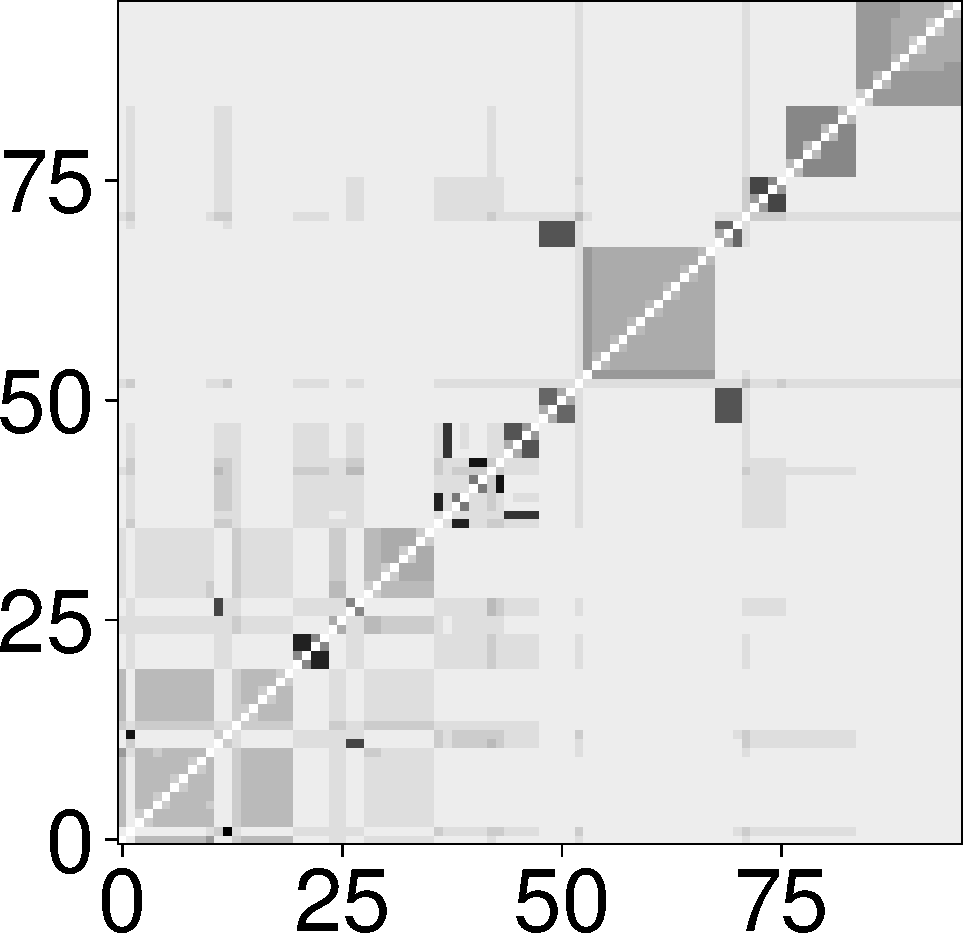
\includegraphics[width=\oneFPage\textwidth]{figures/mechanism/matrices/xeon/redblacktree_96.pdf}
	}
	\subfigure[hashmap]{
		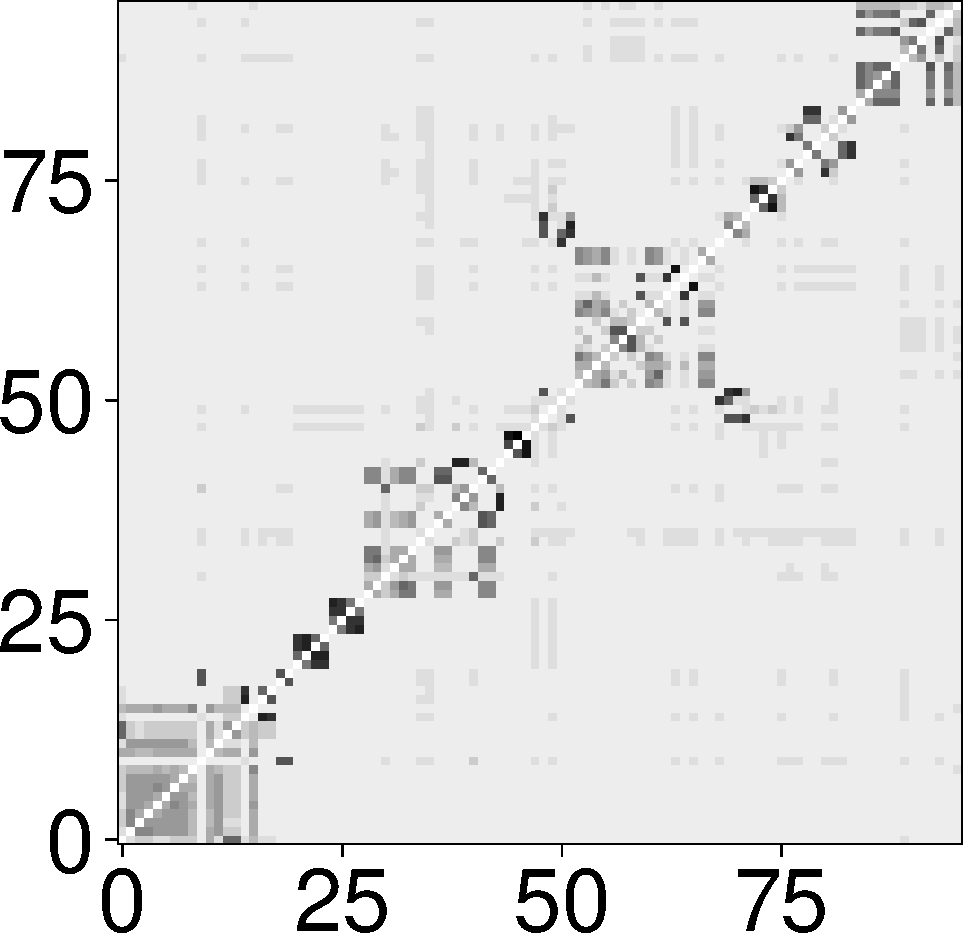
\includegraphics[width=\oneFPage\textwidth]{figures/mechanism/matrices/xeon/hashmap_96.pdf}
	}
	\caption{Communication matrices - 96 threads.}
	\label{fig:commMatrXeon96}
\end{figure}



The two micro-benchmarks (HashMap and Redblacktree) present a communication pattern where neighbor threads communicate often. In that case, darker cells are localized closer to the main diagonal of the matrix. For this pattern, it is interesting to map threads on sibling cores to share all cache levels. On \emph{Genome}, only threads with higher IDs communicates often. Applications such as \emph{ssca2} and \emph{vacation} have an intense communication with all threads, know as all-to-all pattern~\cite{Williams:2009}. On the other hand, \emph{labyrinth} and \emph{bayes} present low communication intensity, but they are considered as an all-to-all pattern as well.


\subsection{Overhead}
To compare the overhead generated by tracking and generating the communication matrices, we compare our mechanism with a memory tracing tool called \texttt{numalize}~\cite{Diener2015}. For some applications \texttt{numalize} crashes and it is not possible the extract the communication matrix. This problem was also observed in others studies that have used this tool~\cite{Soomro:2018}: ``\textit{Unfortunately, in some cases, Numalize crashes because of the large memory requirements of an application in addition to its own internal data structures}''.
Hence, we were only able to run \emph{kmeans} using \texttt{numalize}.

\texttt{Numalize} depends on Intel's \texttt{Pin} tool~\cite{Luk:2005} to instrument the application and trace all accessed addresses, not only the ones accessed by the STM system. Therefore, \texttt{numalize} captures a different memory access behavior compared to our mechanism. This is visualized in \figurename~\ref{fig:numalizeCom} which compares the collected matrices of \emph{kmeans} with 32 and 64 threads using both mechanisms. %The MSE between the matrices collected by \texttt{numalize} and our mechanism is 824.72 (32 threads) and 524.97 (64 threads).

\begin{figure}[!ht]
	\centering
	\subfigure[numalize (32thr)]{
		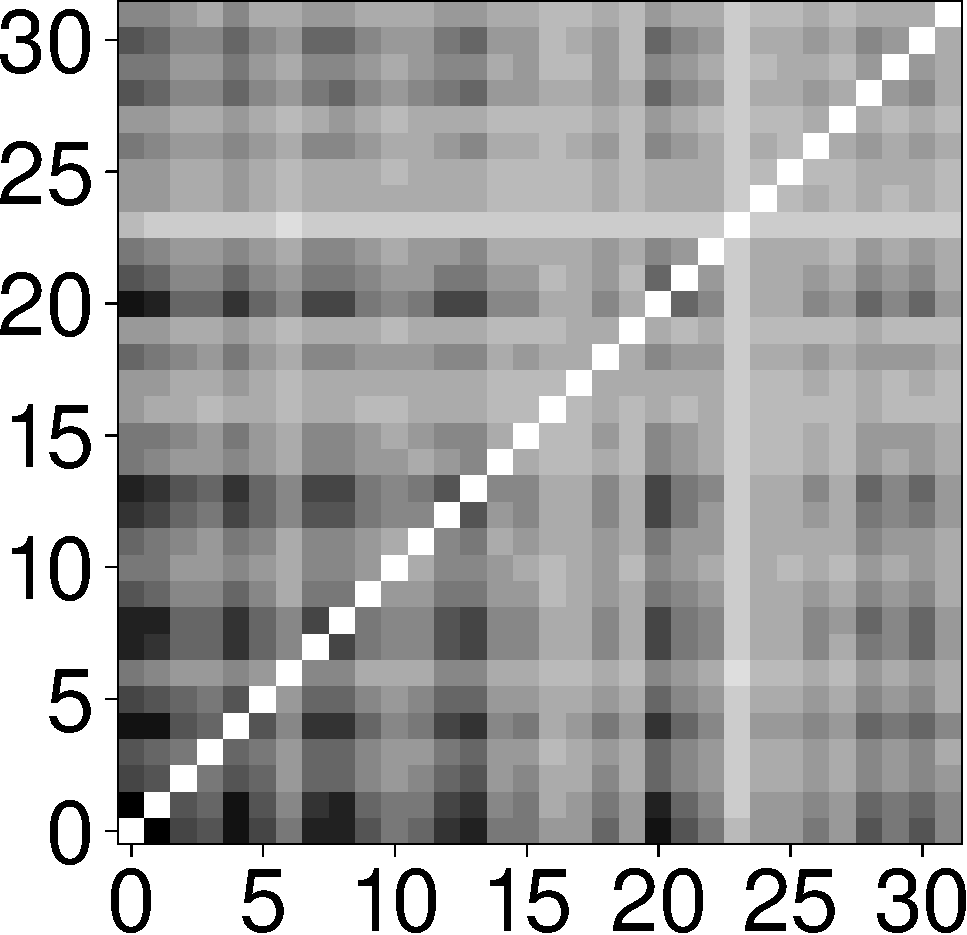
\includegraphics[width=\oneQPage\textwidth]{figures/mechanism/NumalizeC/kmeans.full.6.comm.32.pdf}
	}
	\subfigure[our (32 threads)]{
		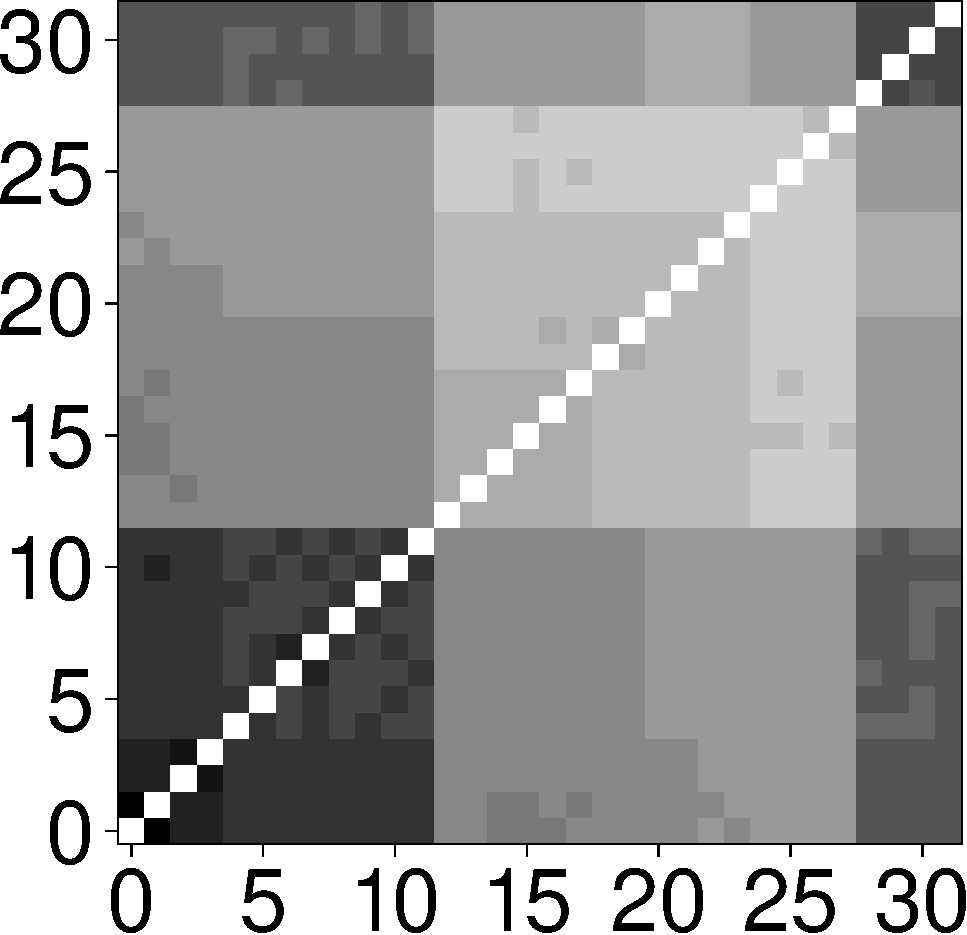
\includegraphics[width=\oneQPage\textwidth]{figures/mechanism/matrices/xeon/kmeans_32.pdf}
	}
	\subfigure[numalize (64thr)]{
		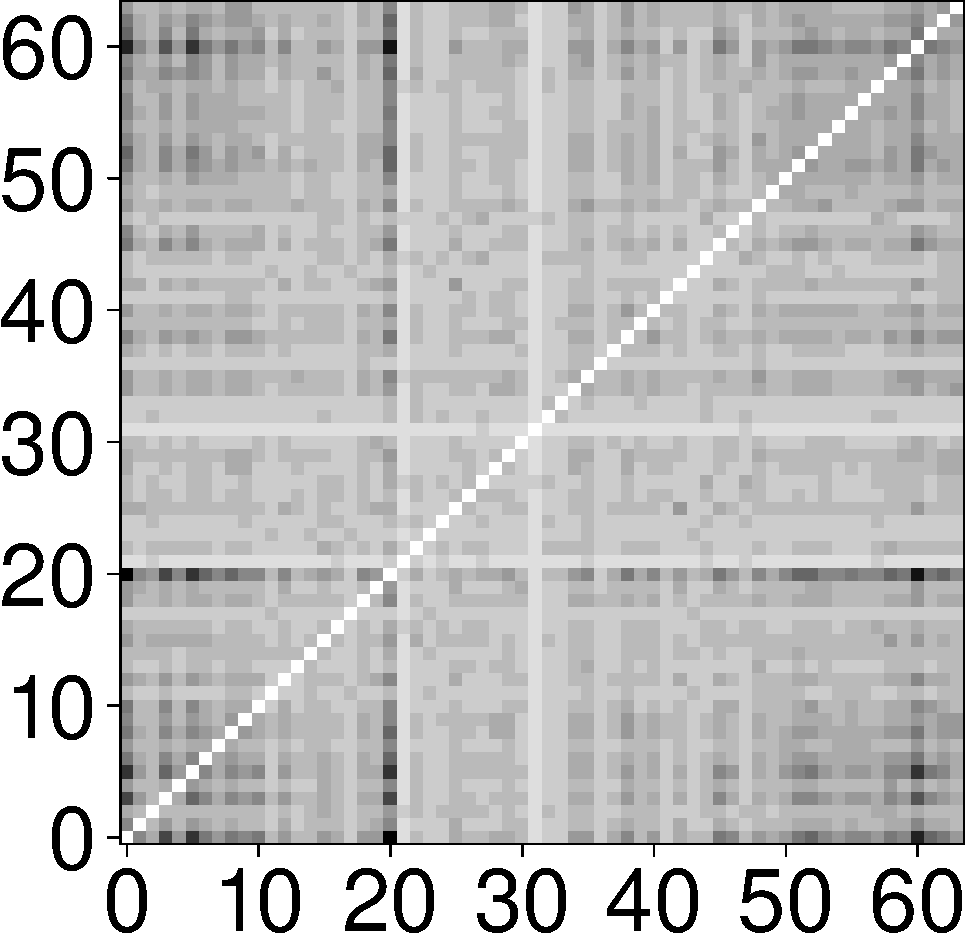
\includegraphics[width=\oneQPage\textwidth]{figures/mechanism/NumalizeC/kmeans.full.6.comm.pdf}
	}
	\subfigure[our (64 threads)]{
		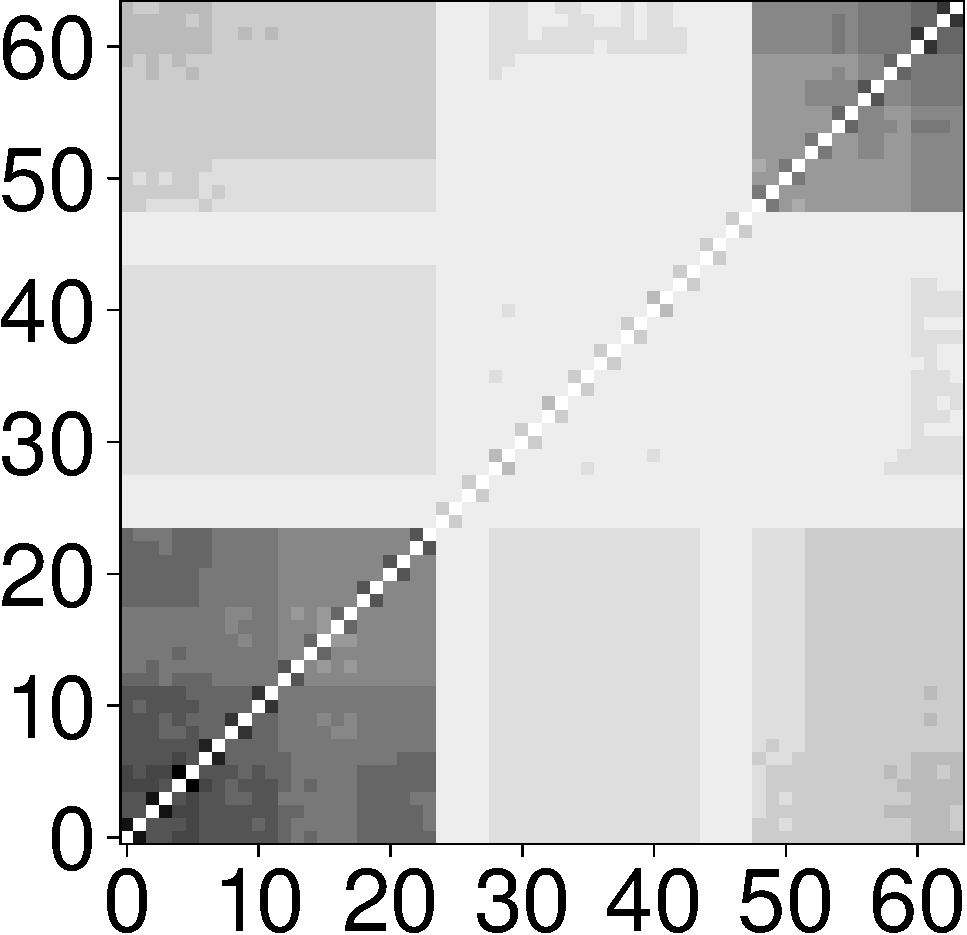
\includegraphics[width=\oneQPage\textwidth]{figures/mechanism/matrices/xeon/kmeans_64.pdf}
	}
	\caption{Comparing \texttt{numalize} and our mechanism on \emph{kmeans}.}
	\label{fig:numalizeCom}
\end{figure}
Another disadvantage of \texttt{numalize} is the overhead added to trace all memory accesses. On \emph{kmeans}, using 64 threads, \texttt{numalize} took 690.90 seconds to execute the application and collect the communication matrix. By contrast, our mechanism took only 46.20 seconds for the same operation, almost 15$\times$ less. The normal execution time for \emph{kmeans} without tracing anything is 18.05 seconds, such that \texttt{numalize} added a overhead of 38.27$\times$, whereas the overhead was 2.5$\times$ with our mechanism. Although the overhead of our mechanism can be considered low, it is unfeasible to be used in an online mechanism. In Section~\ref{sec:lessoverhead}, we will show how to reduce this overhead to be able to perform the detection of sharing behavior during runtime.

%Use the graph of SBAC-PAD (sampling interval 0) to show the added overhead for each application, for collection the matrix.

\section{Summary}

This chapter presented a mechanism to detect the sharing behavior of STM applications. Since STM runtimes need the memory address on each data access operation and have precise information about shared variables, it is possible to determine the communication behavior by tracking transactional reads and writes instead of all memory accesses. Using the proposed mechanism it was possible to extract the sharing behavior of STM applications with lower overhead than other memory trace tools, such as \texttt{numalize}. Although the proposed mechanism has lower overhead, additional experiments are necessary to verify if the collected information is accurate, for instance, if they can be used to calculate an efficient thread mapping. These experiments will be made in Chapter~\ref{chap:sharAwareThreadMap}.
